\section{Results and Analysis}
\label{sec:results}

This section presents overall and per-class classification performance (Section~\ref{sec:methods}.1), a grounded failure-case analysis, a comparative heatmap analysis across all five methods, and quantitative results for cross-replicate explanation consistency, faithfulness, stability, sanity checking, calibration, and shortcut auditing.

\subsection{Classification performance}

Classification performance is reported for the primary-model configuration (Table~\ref{tbl:2}) on the held-out validation split described in Section~\ref{sec:methods}.1.

\begin{table}[!ht]
\centering
\caption{Overall Classification Performance, Primary-Model Configuration (seed~=~42).}
\label{tbl:3}
\begin{tabular}{lc}
\toprule
Metric & Value \\
\midrule
Accuracy & \textbf{0.9305} \\
Macro-F1 & \textbf{0.9303} \\
Macro AUC-ROC & \textbf{0.9965} \\
Validation $n$ & 3193 \\
\bottomrule
\end{tabular}

\vspace{2pt}
\raggedright\footnotesize A three-seed replication (seeds~7, 42, 123; identical architecture, optimizer, and epoch budget) gives accuracy~$0.9210\pm0.0131$, macro-F1~$0.9207\pm0.0131$, macro AUC-ROC~$0.9948\pm0.0023$ (mean~$\pm$~std, $n=3$).
\end{table}

\textbf{Paired statistical significance, three-seed replication.} McNemar's exact test \cite{ref49} on paired per-image accuracy is the primary significance test here, since it directly compares two classifiers' predictions on the same held-out images: the seed~7-vs-seed~42 difference (0.9264 vs.\ 0.9305) is \textit{not} significant ($p=0.451$), while both comparisons involving seed~123 are ($p<0.001$ each, uncorrected for the 3 pairwise seed comparisons tested). DeLong's test \cite{ref47} was also run on per-class, one-vs-rest AUC (1 of 9 classes differs significantly between seed~7 and seed~42, versus 5 of 9 for each comparison involving seed~123, again uncorrected across the resulting 9-class~$\times$~3-seed-pair family of tests) and points in the same qualitative direction, but DeLong's test is designed to compare two correlated ROC curves evaluated on identical patients, not two independently trained models' predictions on the same image set; it is reported here as a secondary, exploratory check rather than the basis for any claim, precisely because that assumption does not hold across independently seeded training runs. Bootstrap 95\% confidence intervals \cite{ref48} (2,000 resamples) come out as seed~7: accuracy $[0.917,\,0.935]$; seed~42: $[0.922,\,0.939]$; seed~123: $[0.895,\,0.915]$; seed~123's interval does not overlap the other two. With only three seeds, however, this is not enough to establish a seed-to-seed distribution or to distinguish a genuinely weaker training run from an unlucky but otherwise typical one; the more defensible claim is only that seed~123 performs measurably worse than the other two \textit{on this specific comparison}, not that it is characteristically different in some reproducible way, and the three-seed mean (92.10\%) should be read alongside all three individual values rather than as a stable population estimate. A separate check asks whether those image-level bootstrap intervals themselves understate uncertainty. Because images sharing a filename-prefix group are correlated rather than independent, a \textit{group} bootstrap (resampling whole filename-prefix groups with replacement, $n=209$ groups over 3,193 validation images, 2,000 resamples) was run alongside the image-level one for all three seeds. The group-aware 95\% accuracy interval comes out 2.7--2.9$\times$ wider than the image-level interval at every seed (seed~7: width 0.018~$\rightarrow$~0.051; seed~42: 0.017~$\rightarrow$~0.046; seed~123: 0.020~$\rightarrow$~0.054), confirming that treating within-group images as independent observations meaningfully understates true uncertainty. The same procedure also reports macro PR-AUC (0.968--0.981) and balanced accuracy (0.909--0.929) per seed, both omitted from the original battery (\texttt{outputs/phase0/group\_aware\_statistics.json}); this is a diagnostic on interval width, not a claim that the point estimates themselves are otherwise incorrect.

Table~\ref{tbl:4} reports the primary model's per-class performance on the held-out validation set (seed~=~42). Unlike the GBCU single-centre dataset examined in prior work (Section~\ref{sec:related-work}), per-class F1 here does not track training-set size closely: the two weakest classes, Perforation (F1~=~0.8944) and Gallstones (F1~=~0.9001), are mid-sized (1,062 and 1,326 total images respectively), while the smallest class, Wall Thickening (990 images), reaches a comfortably higher F1 of 0.9406. These two weakest classes are the primary targets for the failure-case and XAI analysis below.

\begin{table*}[!ht]
\centering
\caption{Per-Class Performance of the Primary Model (9-Class UIdataGB). Classes with low F1 are the primary XAI targets. Best F1/AUC in bold.}
\label{tbl:4}
\begin{tabular}{lcccc}
\toprule
Class & F1 & AUC-ROC & Sensitivity & Specificity \\
\midrule
Gallstones (GS) & 0.9001 & 0.9955 & 0.9373 & 0.9792 \\
Abdomen \& Retroperitoneum (ART) & 0.9161 & 0.9911 & 0.8871 & 0.9936 \\
Cholecystitis (CHOL) & \textbf{0.9601} & 0.9985 & 0.9259 & 0.9996 \\
Membranous/Gangrenous Cholecystitis (MGC) & 0.9428 & 0.9984 & 0.9494 & 0.9919 \\
Perforation (PERF) & 0.8944 & 0.9952 & 0.8469 & 0.9948 \\
Polyps \& Cholesterol Crystals (PCC) & 0.9375 & 0.9958 & 0.8916 & 0.9990 \\
Adenomyomatosis (ADNM) & 0.9360 & 0.9990 & \textbf{1.0000} & 0.9831 \\
Carcinoma (CARC) & 0.9455 & 0.9956 & 0.9404 & 0.9916 \\
Wall Thickening (WT) & 0.9406 & \textbf{0.9996} & 0.9865 & 0.9886 \\
\midrule
\textbf{Macro Avg} & \textbf{0.9303} & \textbf{0.9965} & 0.9295 & 0.9913 \\
\bottomrule
\end{tabular}
\end{table*}

\begin{figure*}[!ht]
\centering
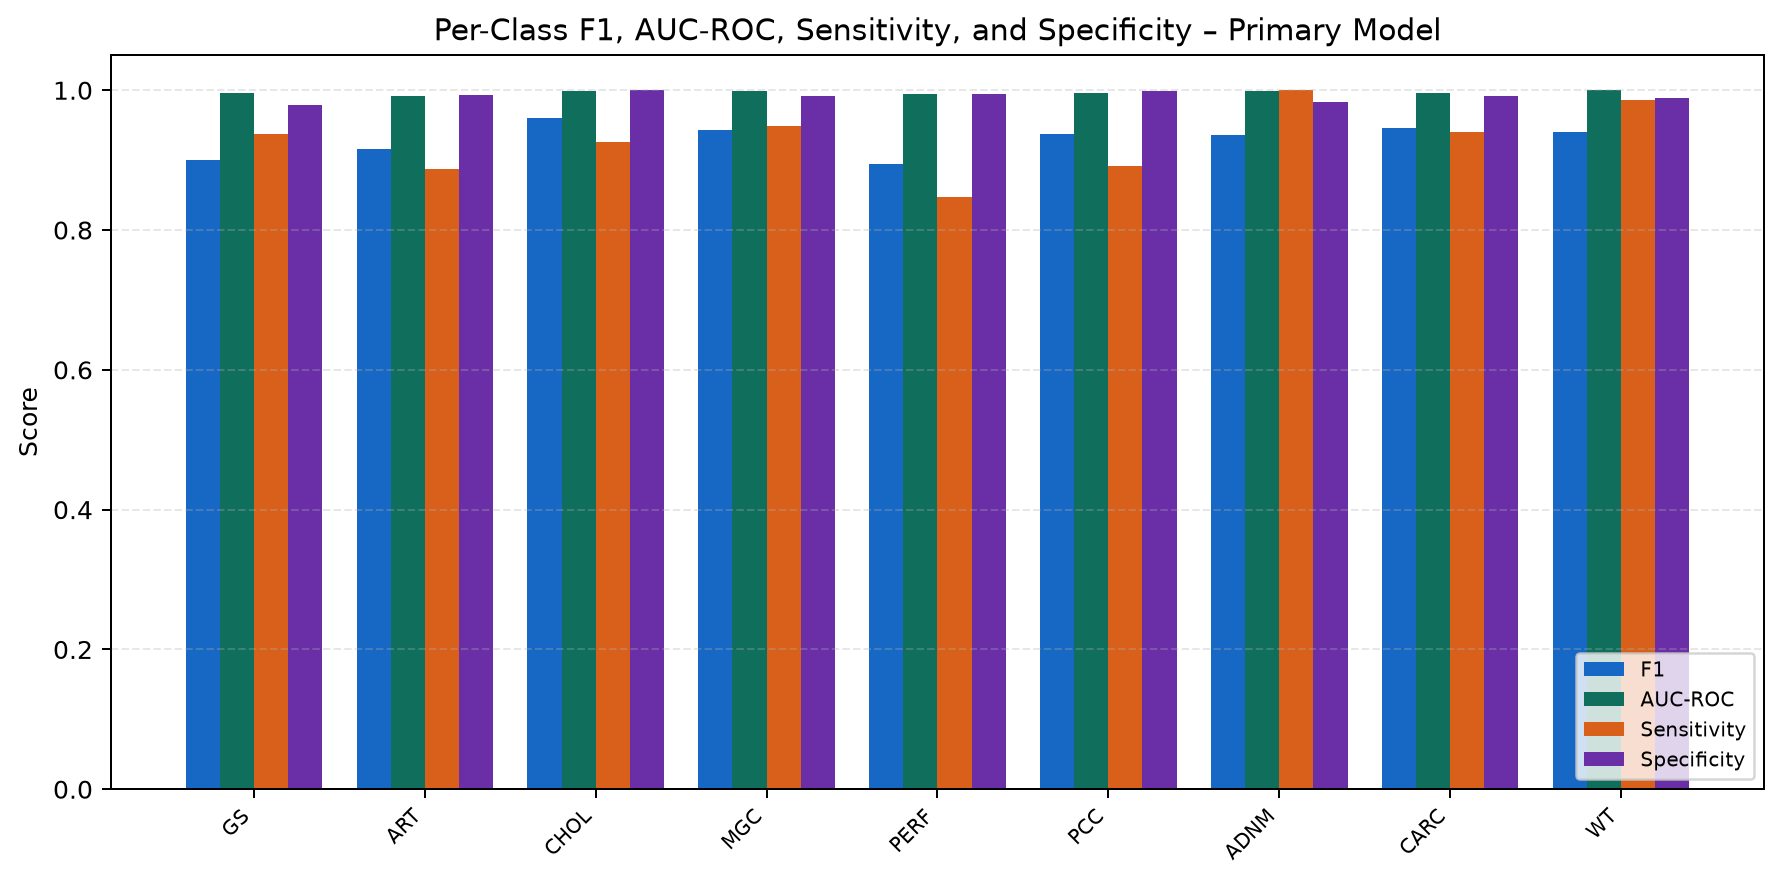
\includegraphics[width=0.75\textwidth]{figures/per_class_metrics.png}
\caption{Per-class F1, AUC-ROC, Sensitivity, and Specificity for the primary model. All nine classes exceed F1~0.89; Perforation and Gallstones are the most challenging by F1, driven by specific confusion pairs (Section~\ref{sec:results}.2) rather than small class size.}
\label{fig:3}
\end{figure*}

\textit{XAI Finding (1):} The per-class performance profile directly informs XAI priorities. Cholecystitis (F1~=~0.9601) and Wall Thickening (AUC~=~0.9996) are the strongest classes and serve as positive controls for anatomical plausibility. Perforation (F1~=~0.8944, sensitivity~0.8469) and Gallstones (F1~=~0.9001) are the most difficult classes---their heatmaps are examined below for whether errors correlate with attention on incorrect anatomical regions.

\begin{figure*}[!ht]
\centering
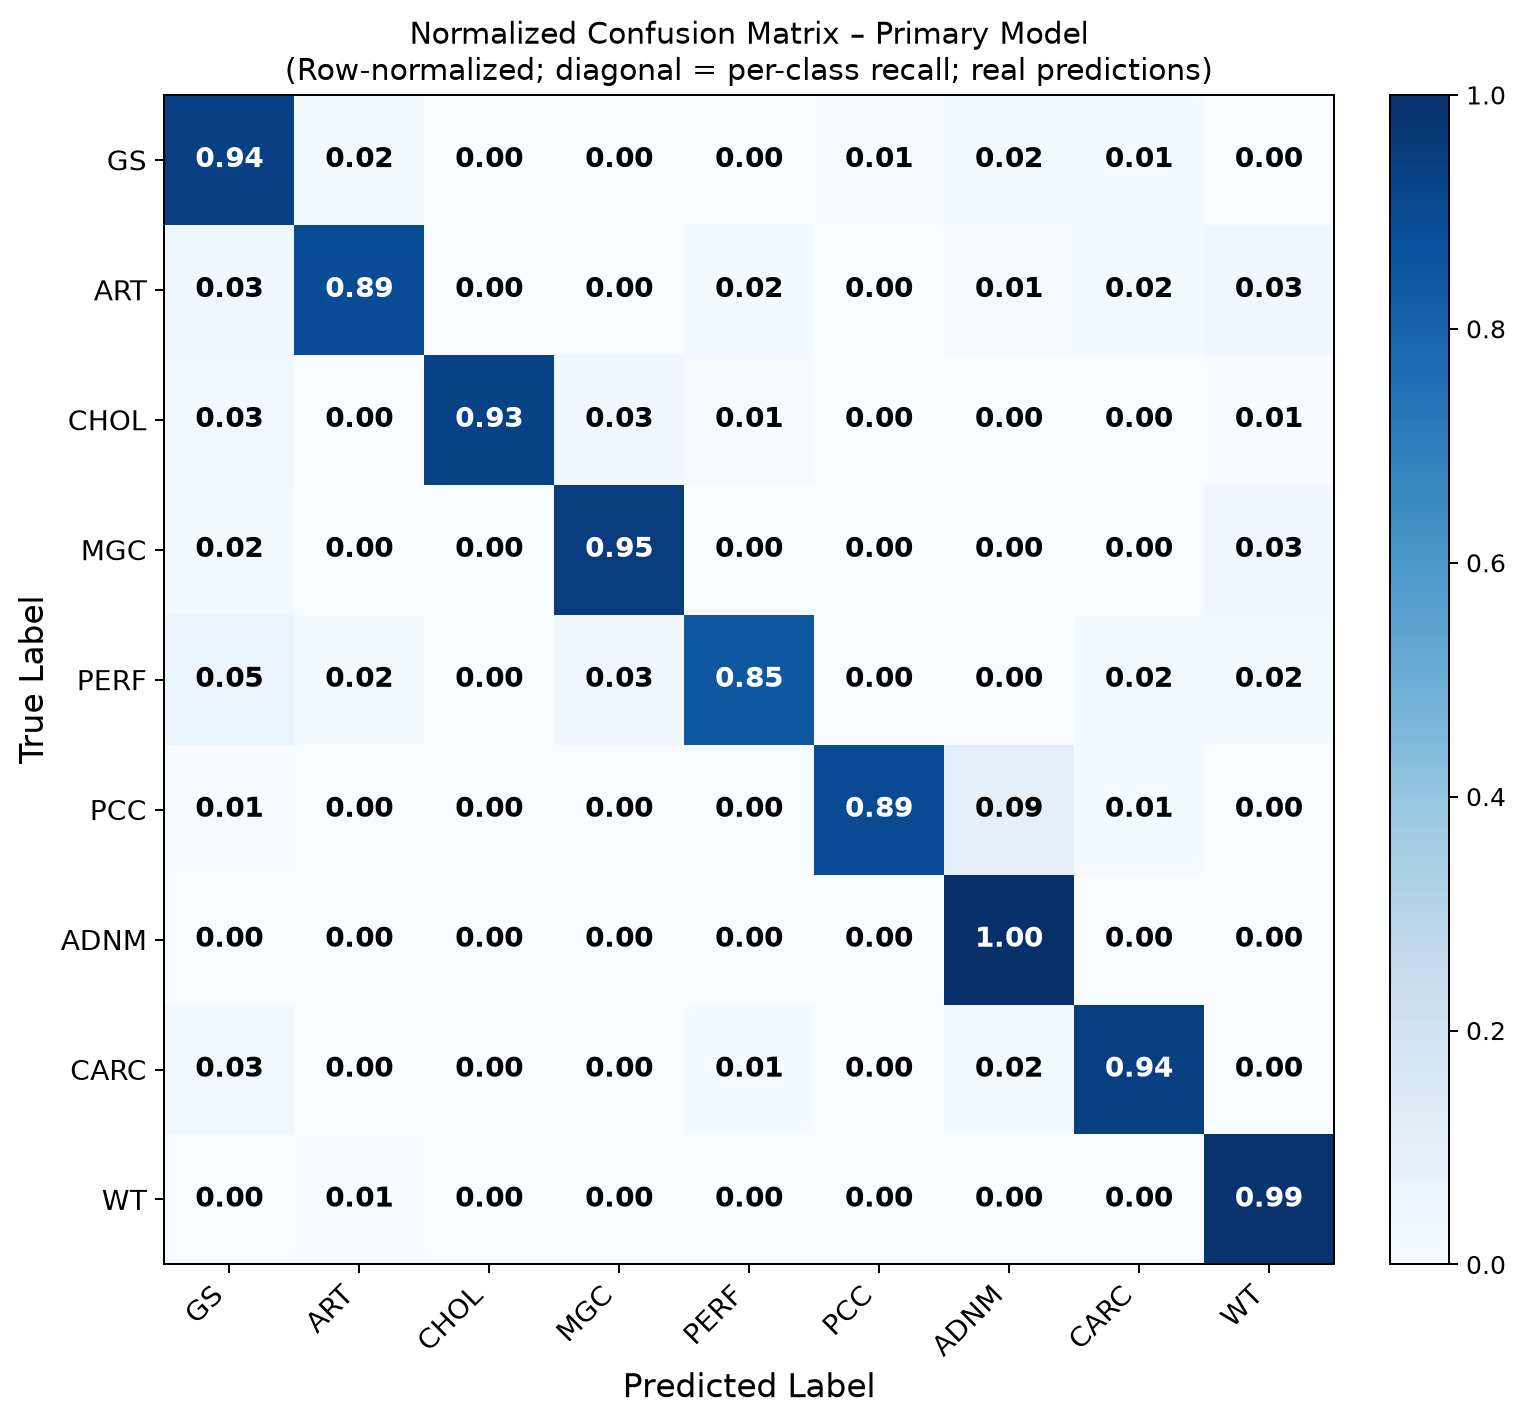
\includegraphics[width=0.42\textwidth]{figures/confusion_normalized}\hfill
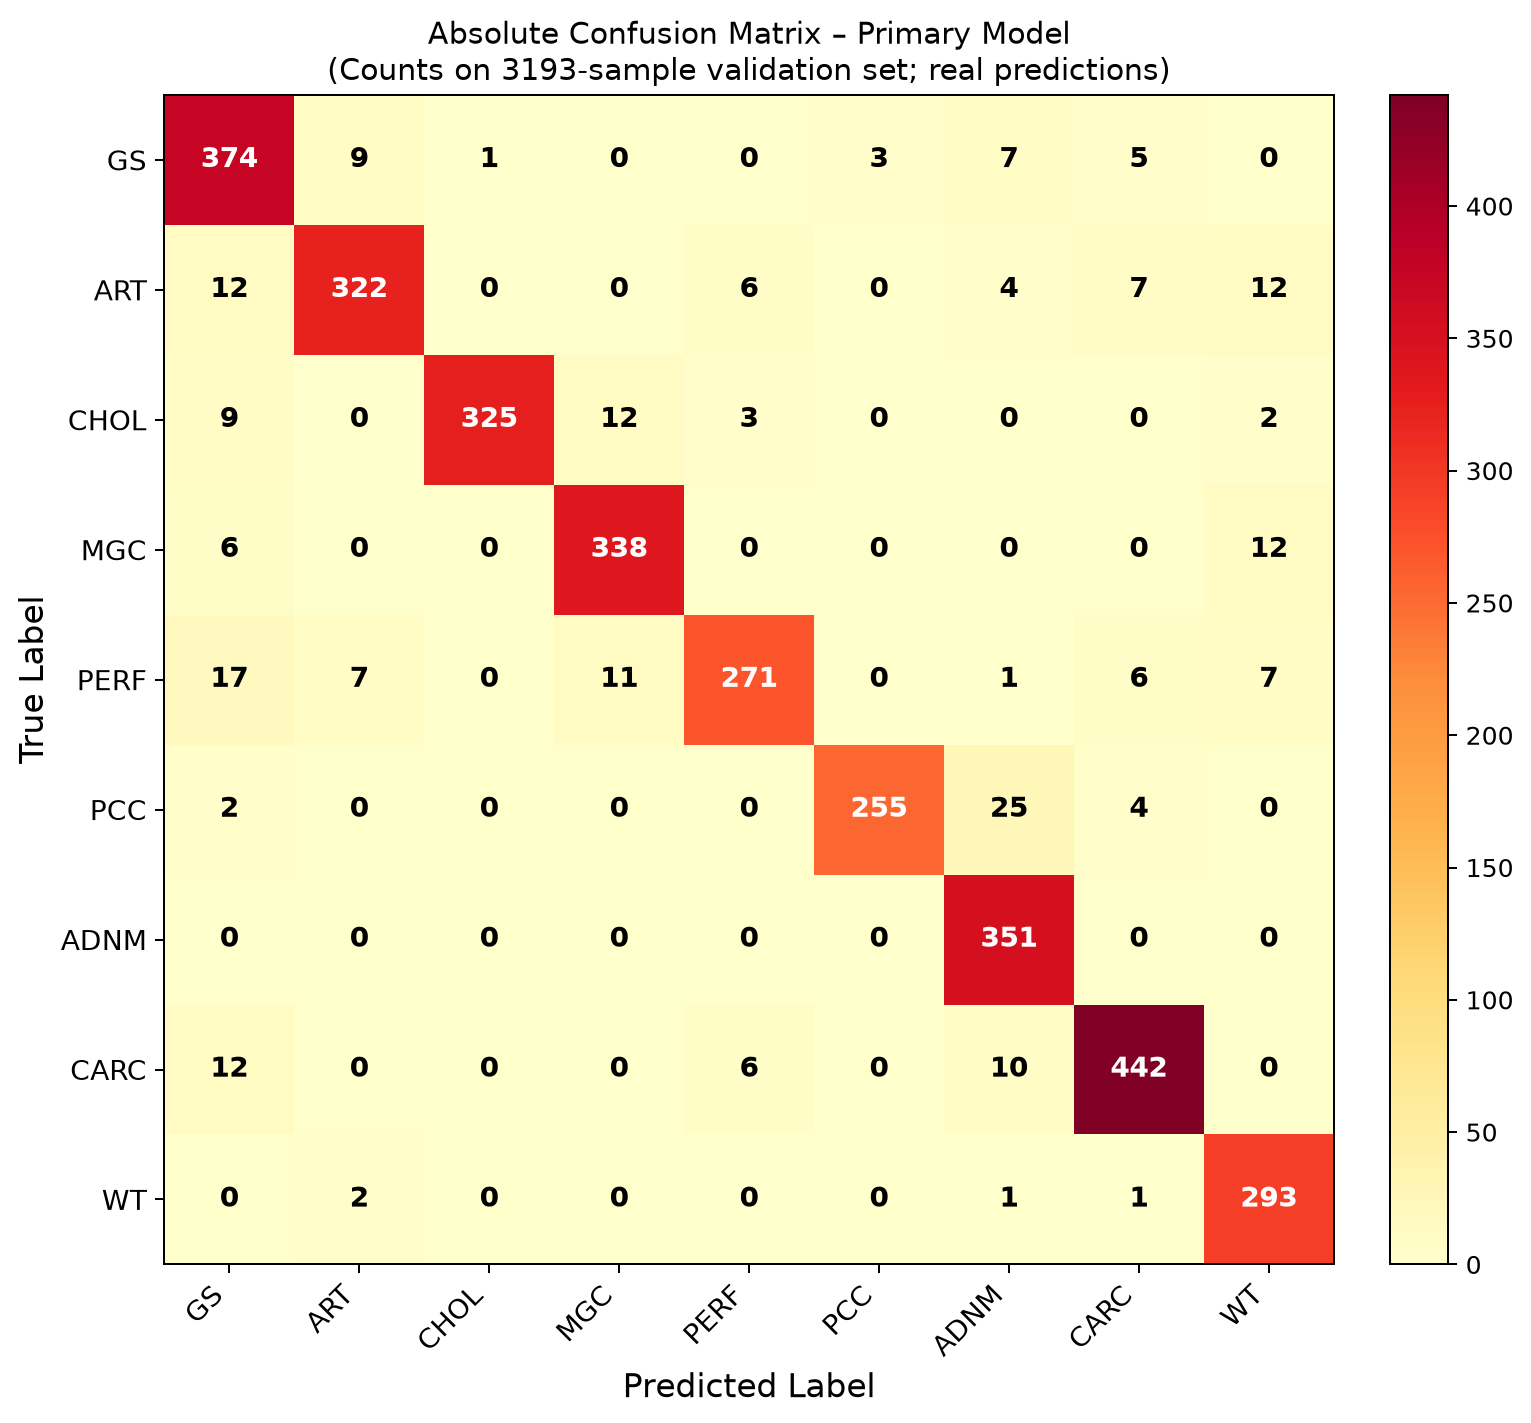
\includegraphics[width=0.42\textwidth]{figures/confusion_absolute}
\caption{(a)~Normalised confusion matrix. Row-normalised values show per-class recall. The largest single confusion is Polyps \& Cholesterol Crystals~$\rightarrow$~Adenomyomatosis. (b)~Absolute confusion matrix. Raw sample counts on the 3,193-image corrected validation set.}
\label{fig:4a}
\end{figure*}

\begin{figure*}[!ht]
\centering
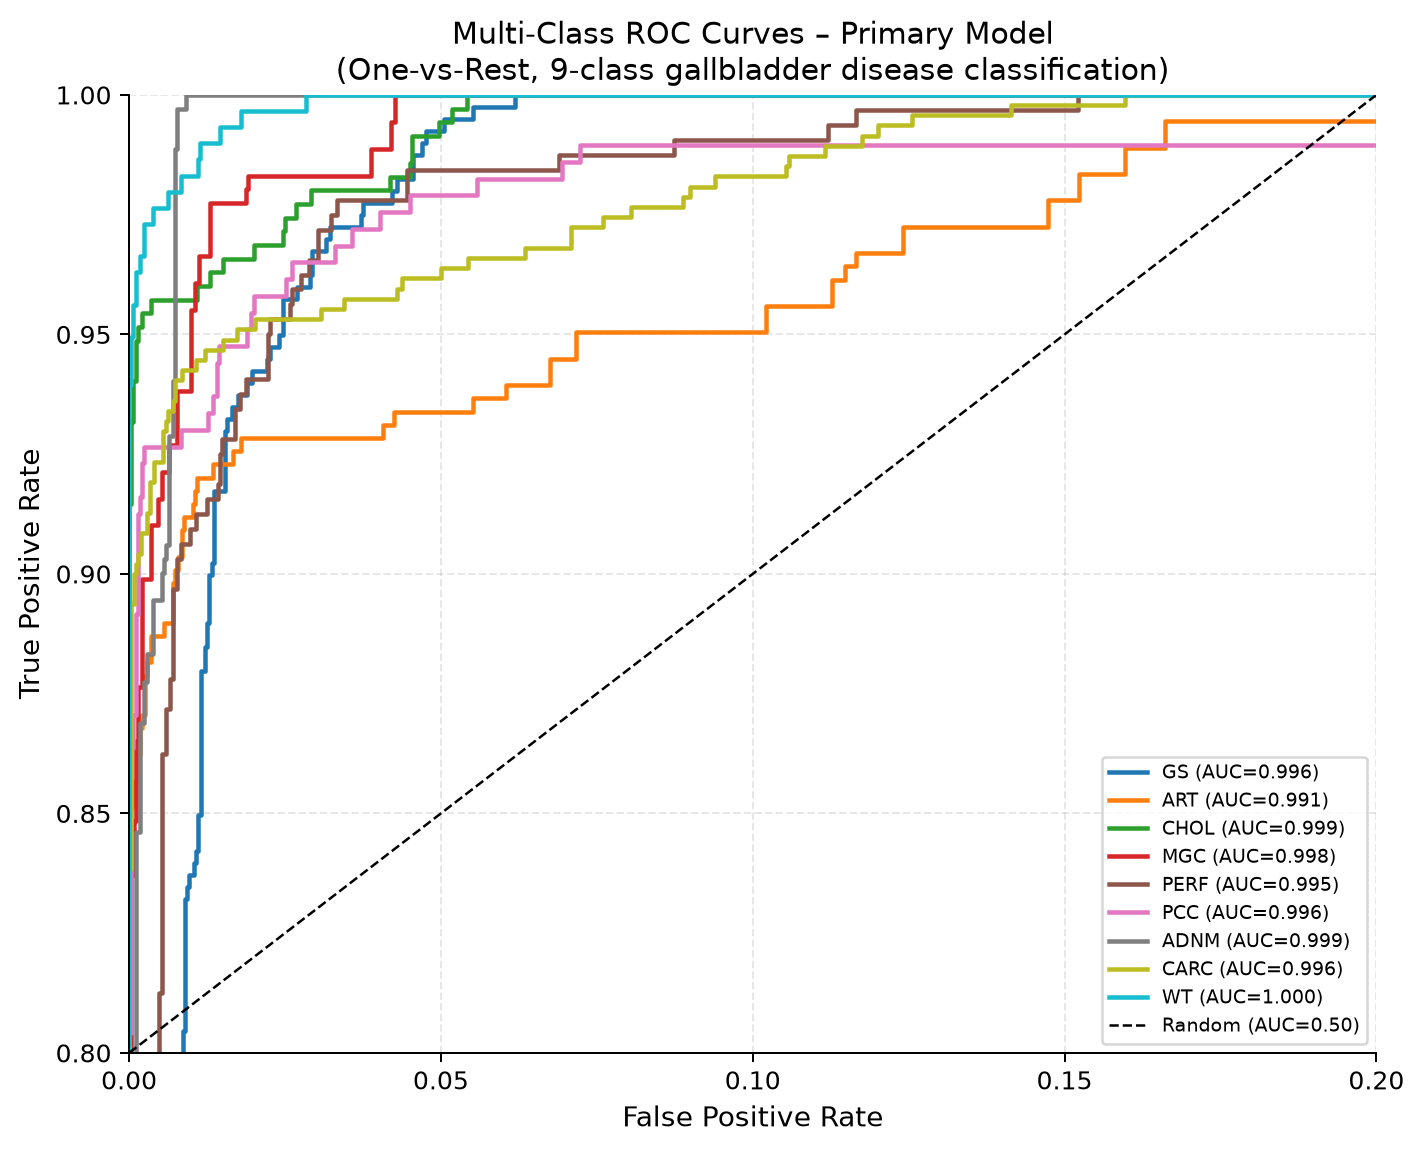
\includegraphics[width=0.6\textwidth]{figures/roc_curves.png}
\caption{One-vs-rest ROC curves for all nine classes. Macro AUC~=~0.9965. Wall Thickening and Adenomyomatosis achieve AUC~$>$~0.999; Abdomen \& Retroperitoneum is lowest at 0.9911, still far above chance.}
\label{fig:5}
\end{figure*}

\subsection{Failure-case analysis}

Of the 3,193 corrected validation images, the model misclassifies 222 (6.95\%), and eight confusion pairs together account for just over half of all errors (113 of 222, 50.9\%): Polyps~\&~Cholesterol Crystals~$\rightarrow$~Adenomyomatosis (25 images), Perforation~$\rightarrow$~Gallstones (17), Abdomen~\&~Retroperitoneum~$\rightarrow$~Gallstones (12), Abdomen~\&~Retroperitoneum~$\rightarrow$~Wall Thickening (12), Cholecystitis~$\rightarrow$~Membranous/Gangrenous Cholecystitis (12), Membranous/Gangrenous Cholecystitis~$\rightarrow$~Wall Thickening (12), Carcinoma~$\rightarrow$~Gallstones (12), and Perforation~$\rightarrow$~Membranous/Gangrenous Cholecystitis (11). Three patterns stand out. The single largest error, Polyps~\&~Cholesterol Crystals~$\rightarrow$~Adenomyomatosis (25 cases), links two benign, morphologically similar entities that both present as echogenic mural foci on ultrasound. Perforation, meanwhile, is confused with Gallstones (17 cases, its single largest error source) and with Membranous/Gangrenous Cholecystitis (11), together accounting for 28 of its total errors, consistent with perforation radiologically overlapping both stone disease and severe gangrenous wall change. A third pattern, Cholecystitis~$\rightarrow$~Membranous/Gangrenous Cholecystitis (12) and Membranous/Gangrenous Cholecystitis~$\rightarrow$~Wall Thickening (12), forms a severity-spectrum confusion chain, the clinically least dangerous direction among the top pairs since all three classes prompt continued attention. Carcinoma~$\rightarrow$~Gallstones (12) is more consequential by contrast: a missed-malignancy error read as benign.

To ground this in specific examples, Fig.~\ref{fig:6} shows two high-confidence wrong predictions from the two weakest classes. A true-Perforation image is classified Gallstones with 99.6\% confidence (the same pattern noted above); its Grad-CAM++ heatmap concentrates on a bright, shadow-adjacent structure, a reasonable-looking but wrong diagnostic cue. A true-Gallstones image is classified Abdomen~\&~Retroperitoneum with 93.6\% confidence, an error direction outside the top eight pairs above. In both cases the model is highly confident despite being wrong, and the heatmap looks anatomically plausible rather than obviously off-target, so heatmap plausibility alone would not have flagged either error. That is a real limitation of plausibility as an error-detection signal on its own (Section~\ref{sec:discussion}.2).

\begin{figure*}[!ht]
\centering
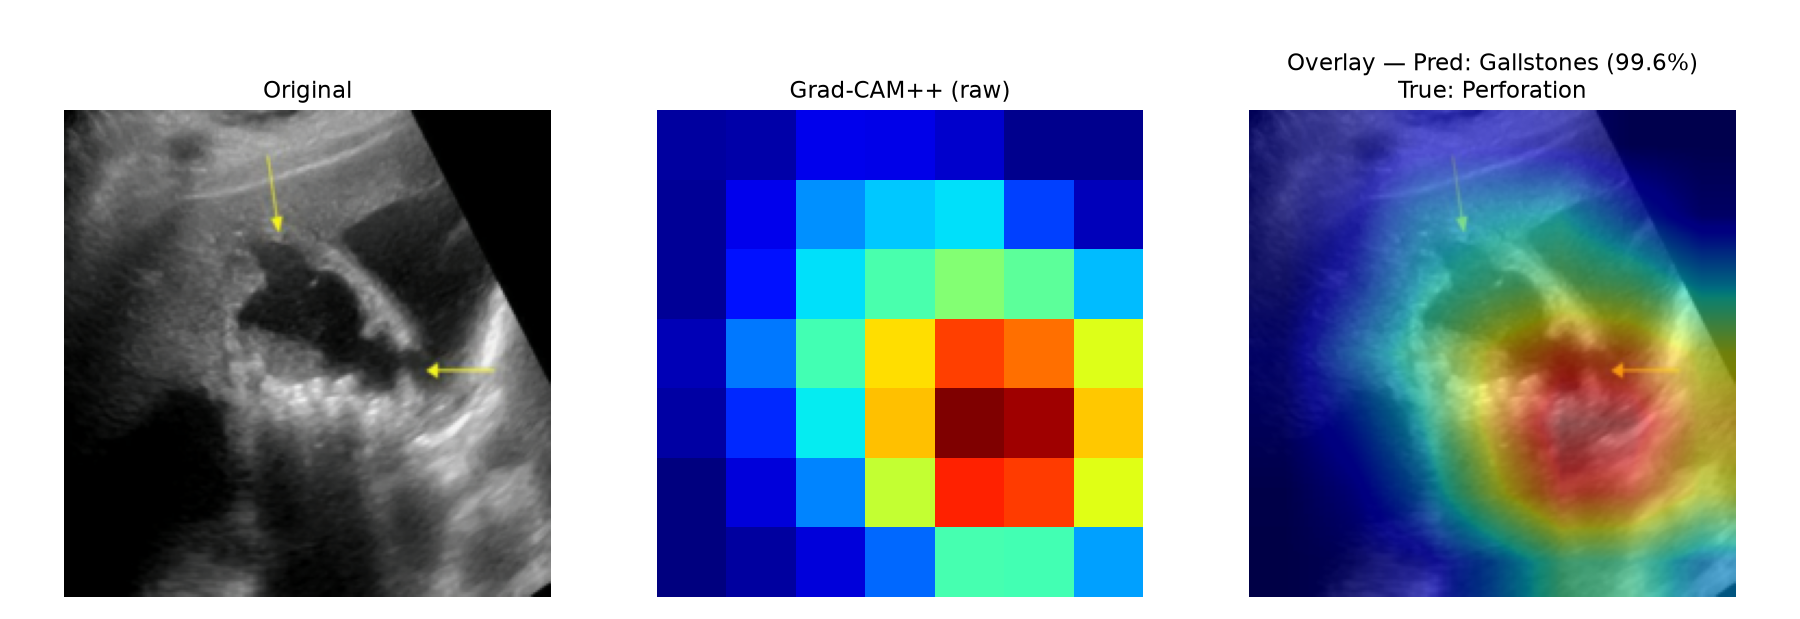
\includegraphics[width=0.42\textwidth]{figures/failure_case_perforation}\hfill
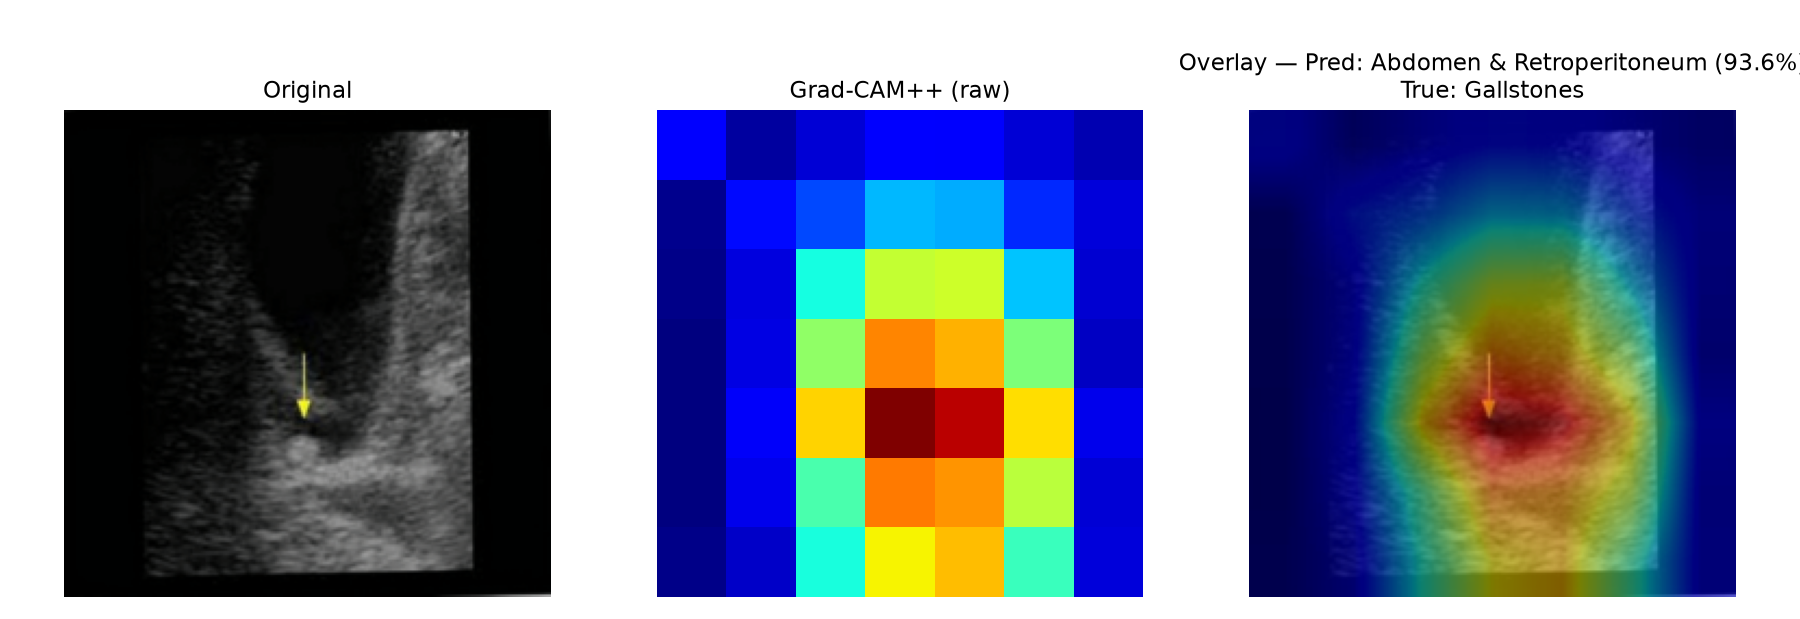
\includegraphics[width=0.42\textwidth]{figures/failure_case_gallstones}
\caption{Two representative high-confidence misclassifications, one from each of the two weakest classes (Table~\ref{tbl:4}). Left: true Perforation predicted Gallstones (99.6\%) --- the single largest confusion-pair direction for Perforation (Pattern~2). Right: true Gallstones predicted Abdomen~\&~Retroperitoneum (93.6\%). Each panel shows the original ultrasound, the Grad-CAM++ heatmap, and the overlay. Both heatmaps are anatomically plausible-looking despite the wrong label, illustrating that heatmap plausibility alone does not reliably flag classification errors.}
\label{fig:6}
\end{figure*}

\textbf{Confidence and calibration signal (uncalibrated).} Mean softmax confidence is 0.974 on correctly classified images but 0.771 on misclassified ones, suggesting a confidence-threshold triage could surface many mistakes for review. This is only a raw-softmax observation, though, and raw softmax confidence is known to be an unreliable proxy for true probability \cite{ref42}; the miscalibration it points to is quantified and formally corrected (ECE, Brier score, temperature scaling) in Section~\ref{sec:results}.4.

\subsection{Qualitative and quantitative comparison of XAI methods}

All five XAI methods are applied to the primary model across all nine disease classes. \textbf{Grad-CAM} produces smooth, region-level heatmaps, while \textbf{Grad-CAM++} consistently generates sharper, more focused activation patches, particularly for Carcinoma and Membranous/Gangrenous Cholecystitis, where the discriminative feature is a localised wall irregularity rather than a diffuse region. \textbf{Saliency Maps} highlight fine-grained pixel-level evidence but carry more background noise, and \textbf{Eigen-CAM}, being class-agnostic, highlights the single dominant activation pattern regardless of predicted class, which makes it informative as a sanity baseline but weaker for per-class discrimination. \textbf{Score-CAM} produces heatmaps similar in character to Grad-CAM++, since both explicitly condition on the target class's evidence, one via second-order gradients and the other via masked-input forward passes.

\textit{XAI Finding (2):} Grad-CAM++ and Score-CAM produce noticeably sharper, more class-discriminative localization than Grad-CAM, Saliency, or Eigen-CAM for Carcinoma and Membranous/Gangrenous Cholecystitis, where the discriminative feature is a localised wall structure rather than a broad region. For Cholecystitis and Wall Thickening, all CAM-family methods produce similar heatmaps, consistent with those classes having larger, more uniformly distributed discriminative features.

\textit{XAI Finding (3):} In representative examples across all nine classes, the primary model's Grad-CAM++ attention appears anatomically plausible when inspected visually: acoustic shadow for Gallstones, focal wall attention for Carcinoma, diffuse wall-adjacent change for the mutually-confusable MGC/Perforation pair, small mural foci for the mutually-confusable Adenomyomatosis/PCC pair, and broader body-wide attention for ART and Wall Thickening. This is the authors' visual assessment, not a claim of anatomical correctness validated against clinician-defined regions of interest (Section~\ref{sec:limitations}).

Grad-CAM++ and Score-CAM improve most clearly over Grad-CAM for Carcinoma and Membranous/Gangrenous Cholecystitis, where the model needs to localise subtle wall changes rather than broad regions. Saliency Maps consistently highlight gallbladder boundary pixels, while Eigen-CAM's class-agnostic pattern is visibly less anatomically focused than the other four methods across every row. Supplementary Material A contains the full, non-cherry-picked per-class Grad-CAM++ gallery and a cross-method comparison grid showing all five XAI methods side by side for one representative image per class.

Figs.~\ref{fig:8} and \ref{fig:8b} show, respectively, ten and a further ten representative images spanning all nine classes (two to three per class, 20 in total), each with the original, raw Grad-CAM++ heatmap, overlay, and the model's predicted-class confidence, to confirm the heatmap patterns above are not an artefact of a single cherry-picked image per class. The remaining images of the full 54-image, non-cherry-picked gallery (six samples per class) are in Supplementary Material A.

\begin{figure*}[!ht]
\centering
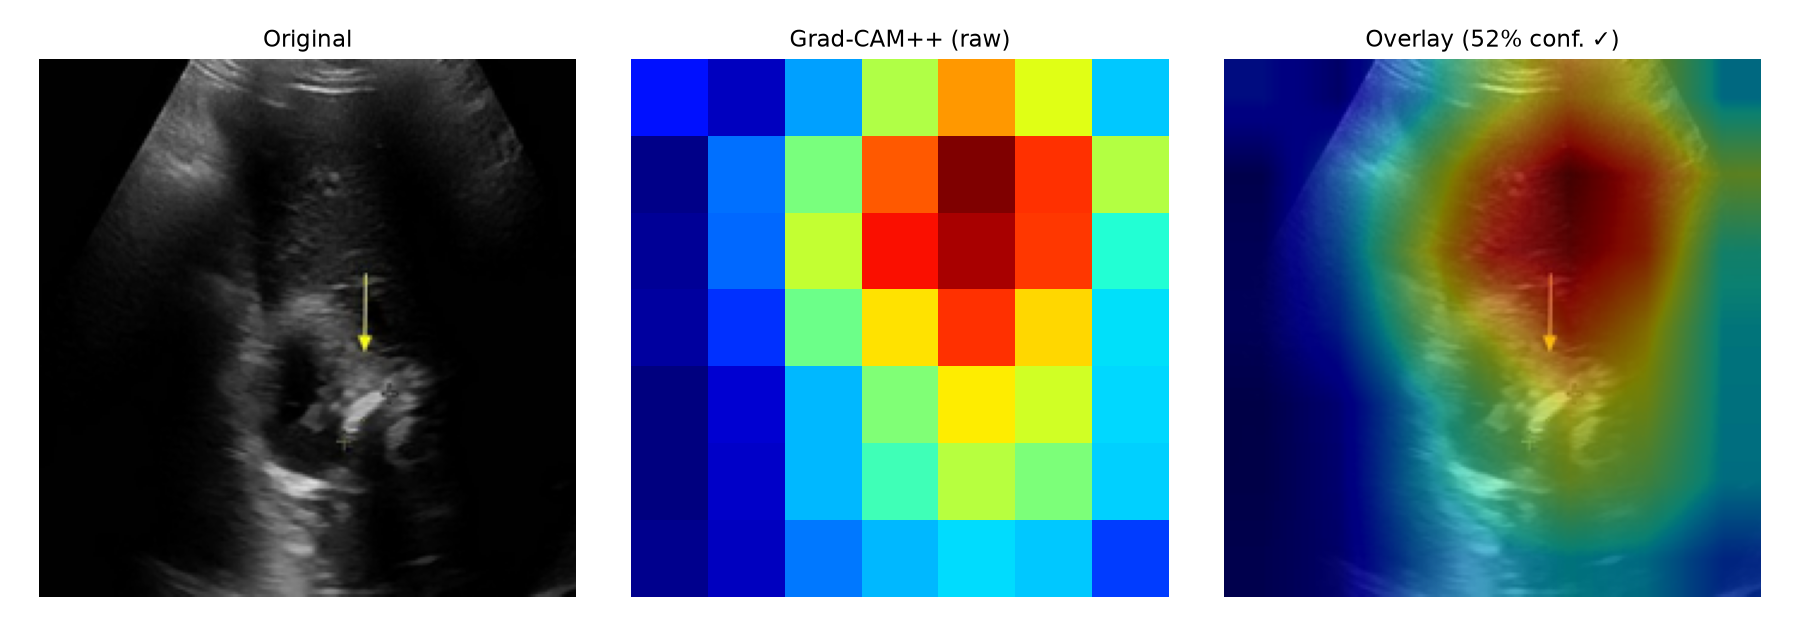
\includegraphics[width=0.48\linewidth]{figures/fig7_expanded/01_gallstones_01}\hfill
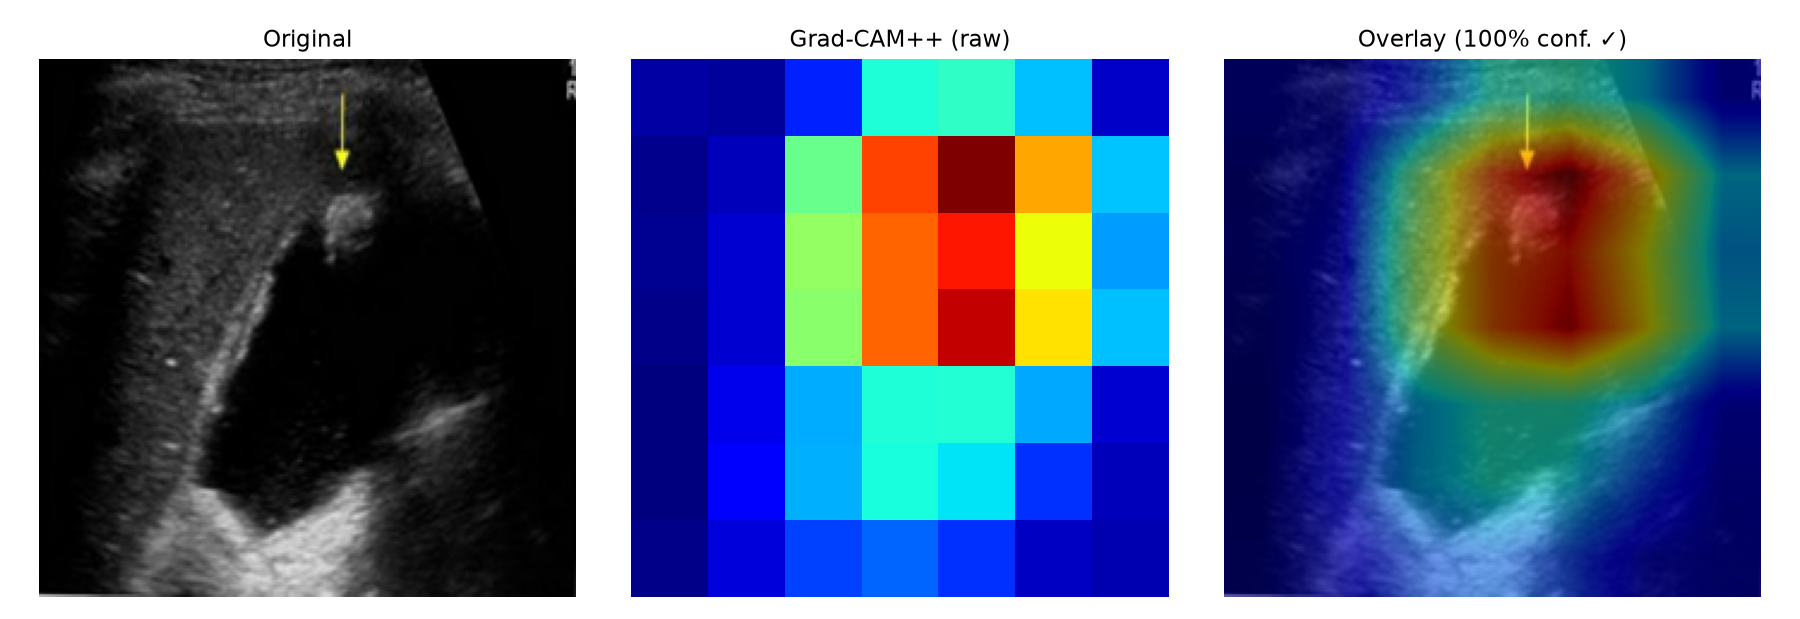
\includegraphics[width=0.48\linewidth]{figures/fig7_expanded/01_gallstones_02}\\[2pt]
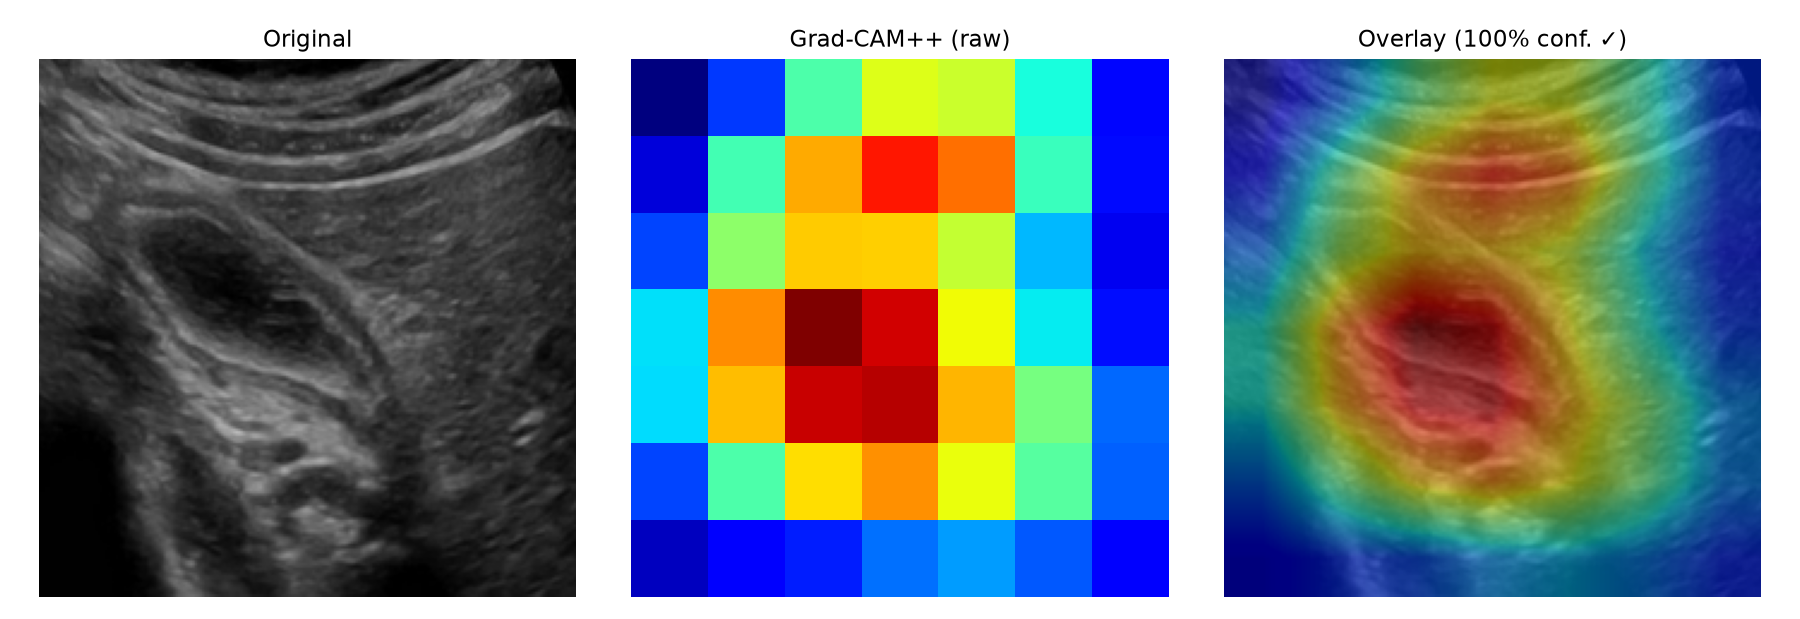
\includegraphics[width=0.48\linewidth]{figures/fig7_expanded/01_gallstones_03}\hfill
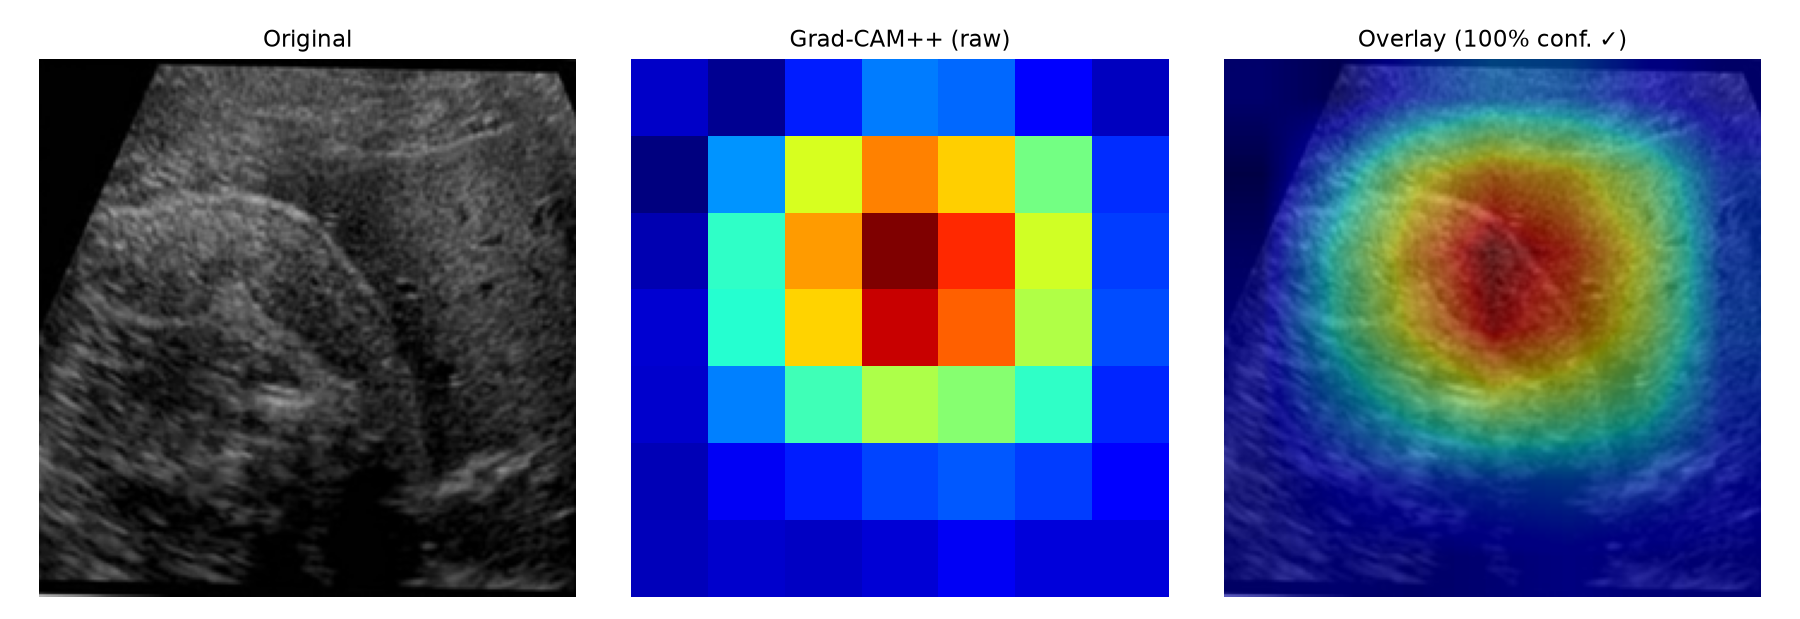
\includegraphics[width=0.48\linewidth]{figures/fig7_expanded/02_abdomen_and_retroperitoneum_01}\\[2pt]
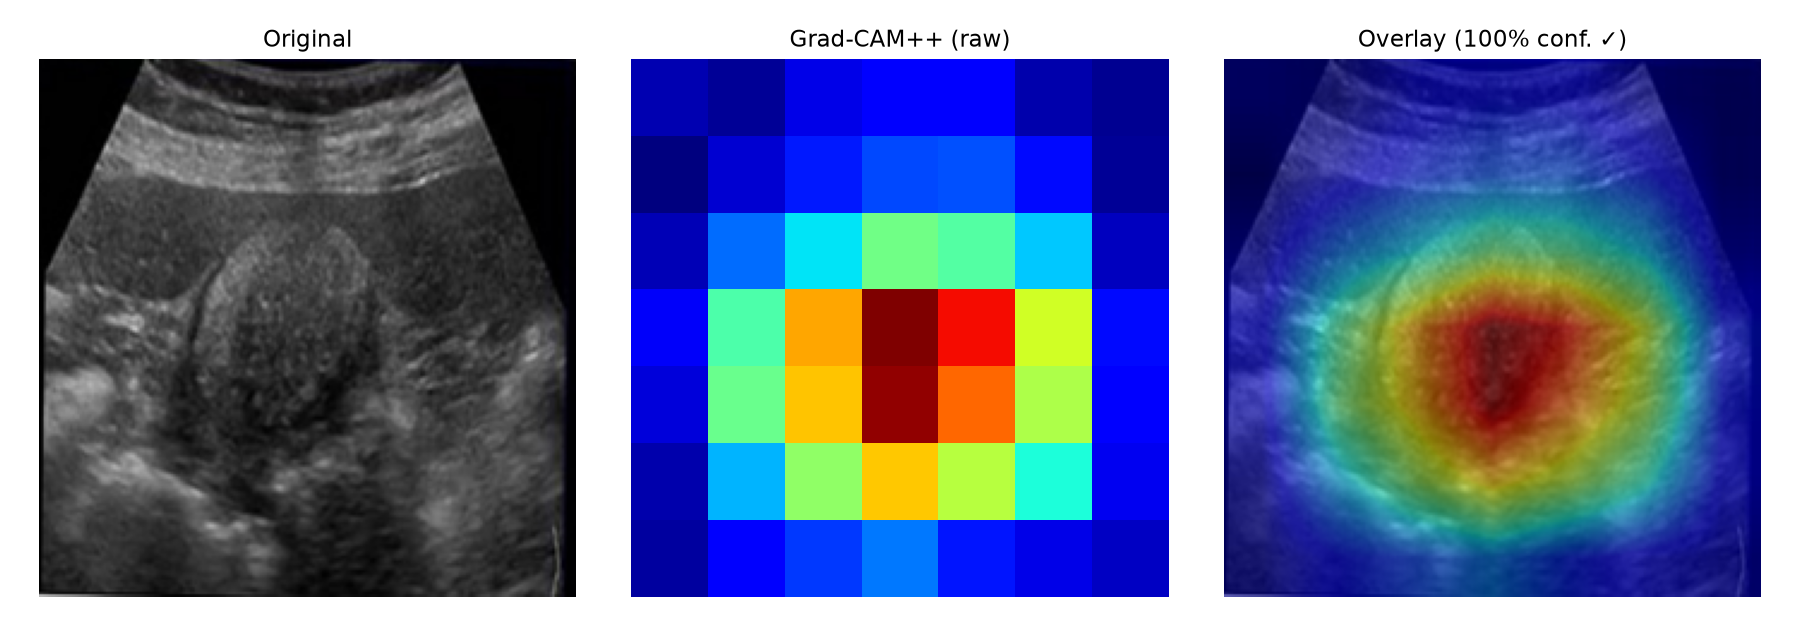
\includegraphics[width=0.48\linewidth]{figures/fig7_expanded/02_abdomen_and_retroperitoneum_02}\hfill
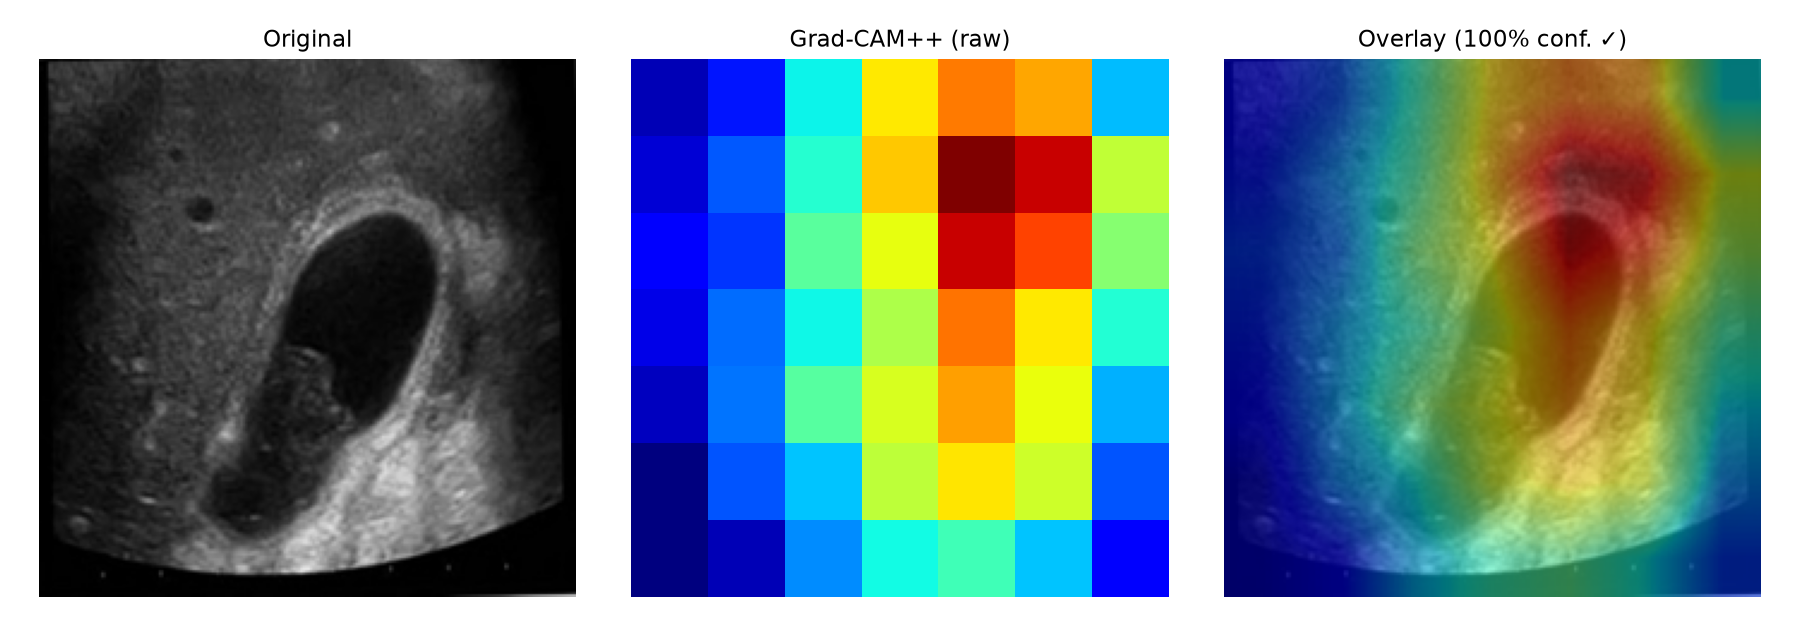
\includegraphics[width=0.48\linewidth]{figures/fig7_expanded/03_cholecystitis_01}\\[2pt]
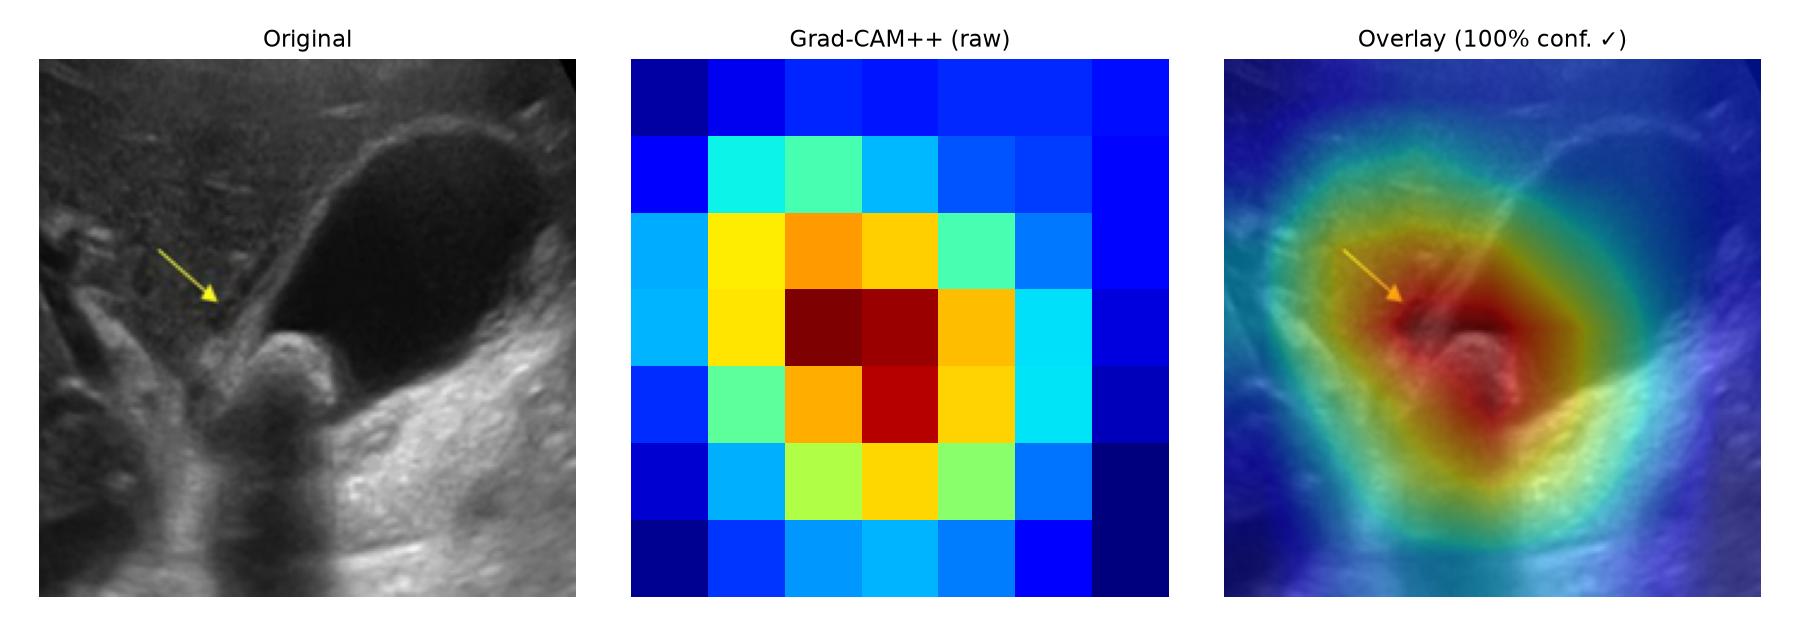
\includegraphics[width=0.48\linewidth]{figures/fig7_expanded/03_cholecystitis_02}\hfill
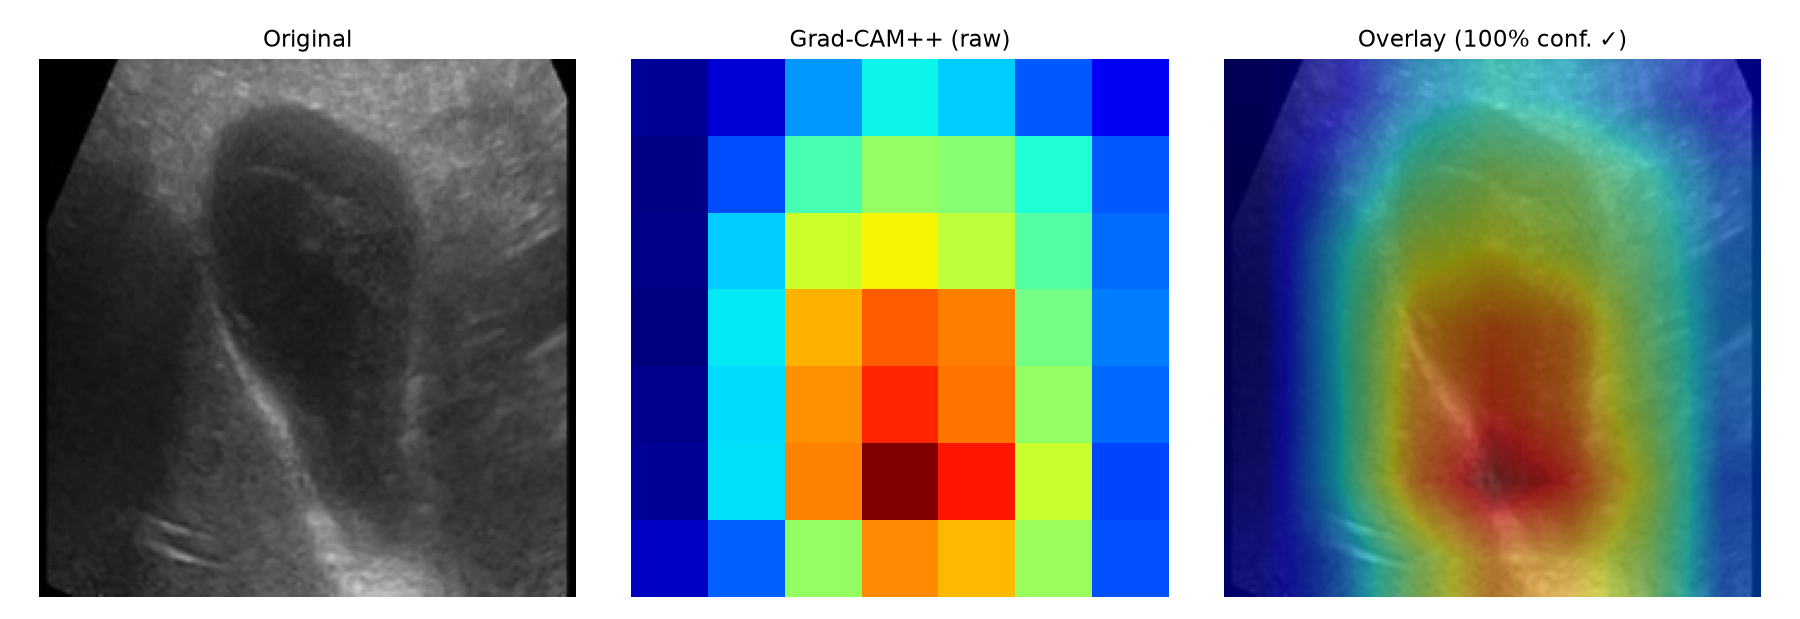
\includegraphics[width=0.48\linewidth]{figures/fig7_expanded/04_membranous_and_gangrenous_cholecystitis_01}\\[2pt]
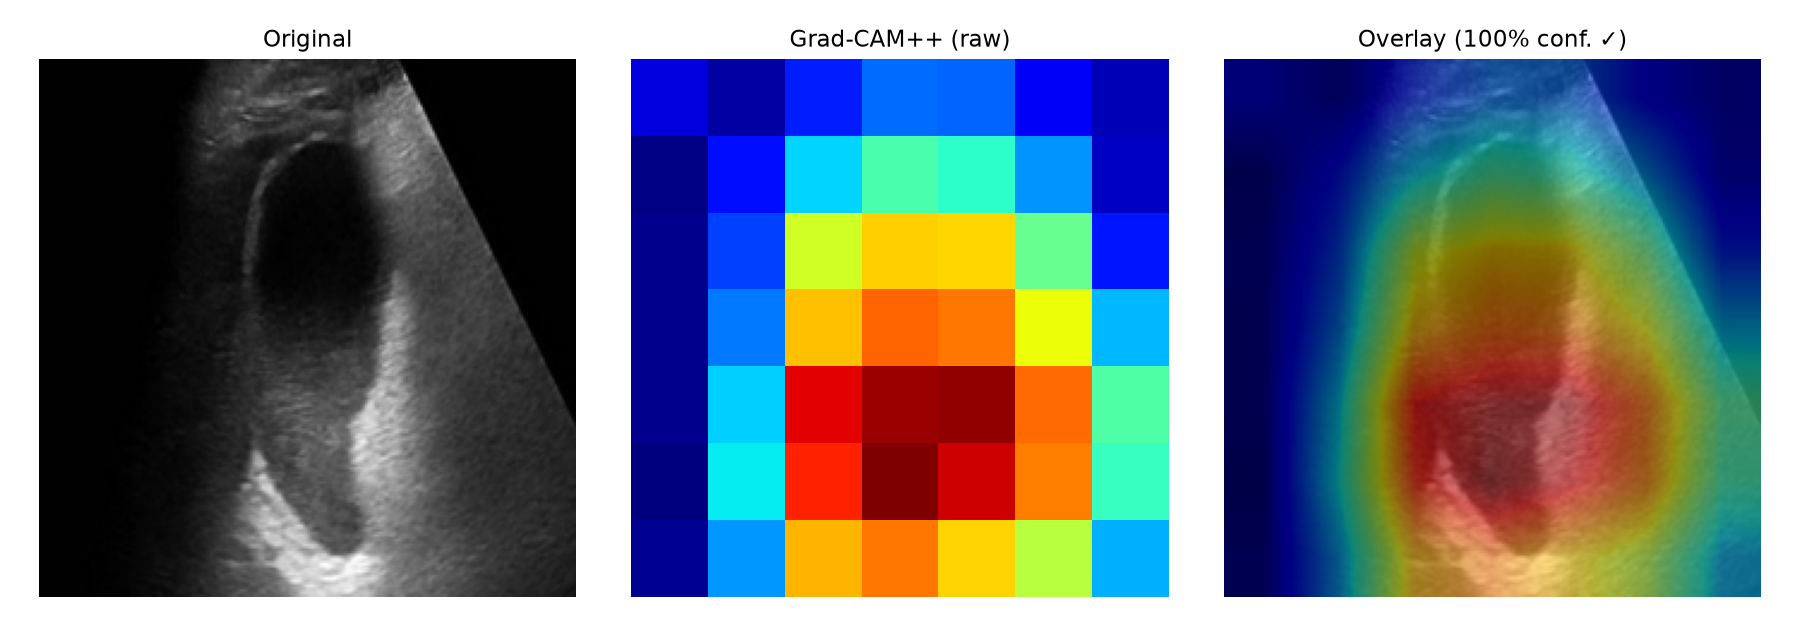
\includegraphics[width=0.48\linewidth]{figures/fig7_expanded/04_membranous_and_gangrenous_cholecystitis_02}\hfill
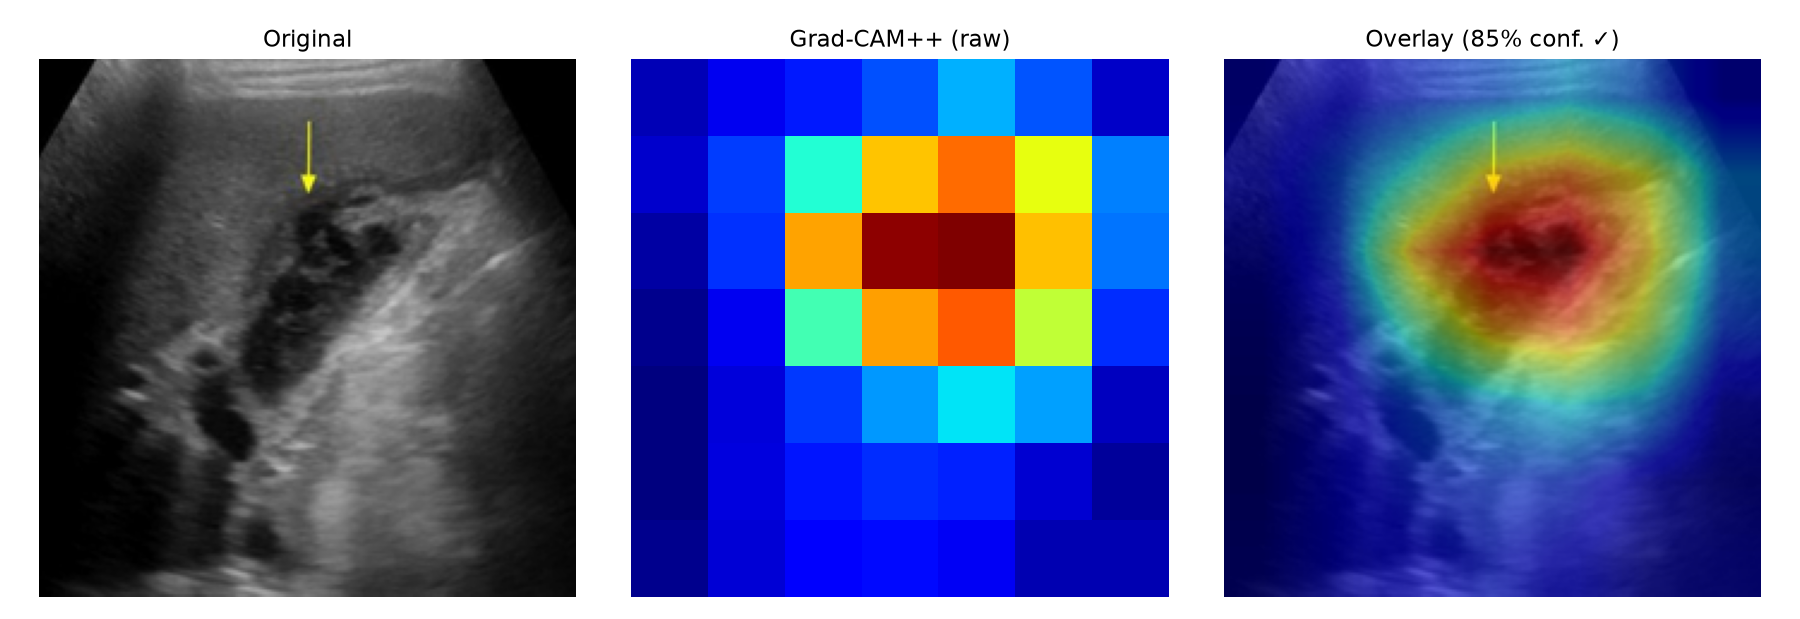
\includegraphics[width=0.48\linewidth]{figures/fig7_expanded/05_perforation_01}
\caption{Original image, raw Grad-CAM++ heatmap, and overlay for two-to-three representative images each of Gallstones, Abdomen \& Retroperitoneum, Cholecystitis, and Membranous/Gangrenous Cholecystitis, plus one of Perforation (continued in Fig.~\ref{fig:8b}). Each overlay panel is labelled with the model's predicted-class confidence and a \checkmark/\ding{55} marker for correctness. Attention concentrates on central image content in the region conventionally associated with the gallbladder wall and lumen, consistent with the class-specific patterns described in Section~\ref{sec:results}.3; this is a visual, non-clinician-validated observation (Section~\ref{sec:limitations}).}
\label{fig:8}
\end{figure*}

\begin{figure*}[!ht]
\centering
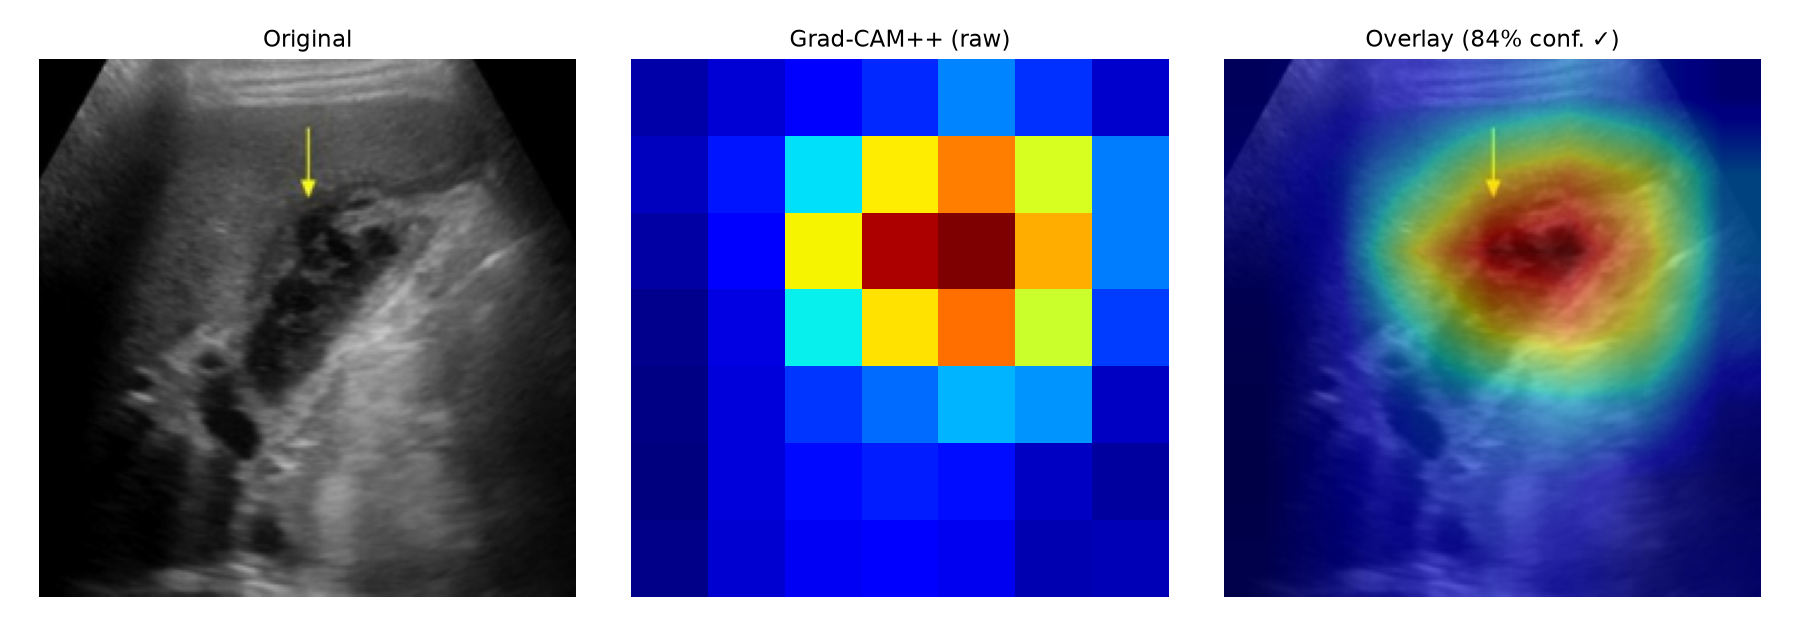
\includegraphics[width=0.48\linewidth]{figures/fig7_expanded/05_perforation_02}\hfill
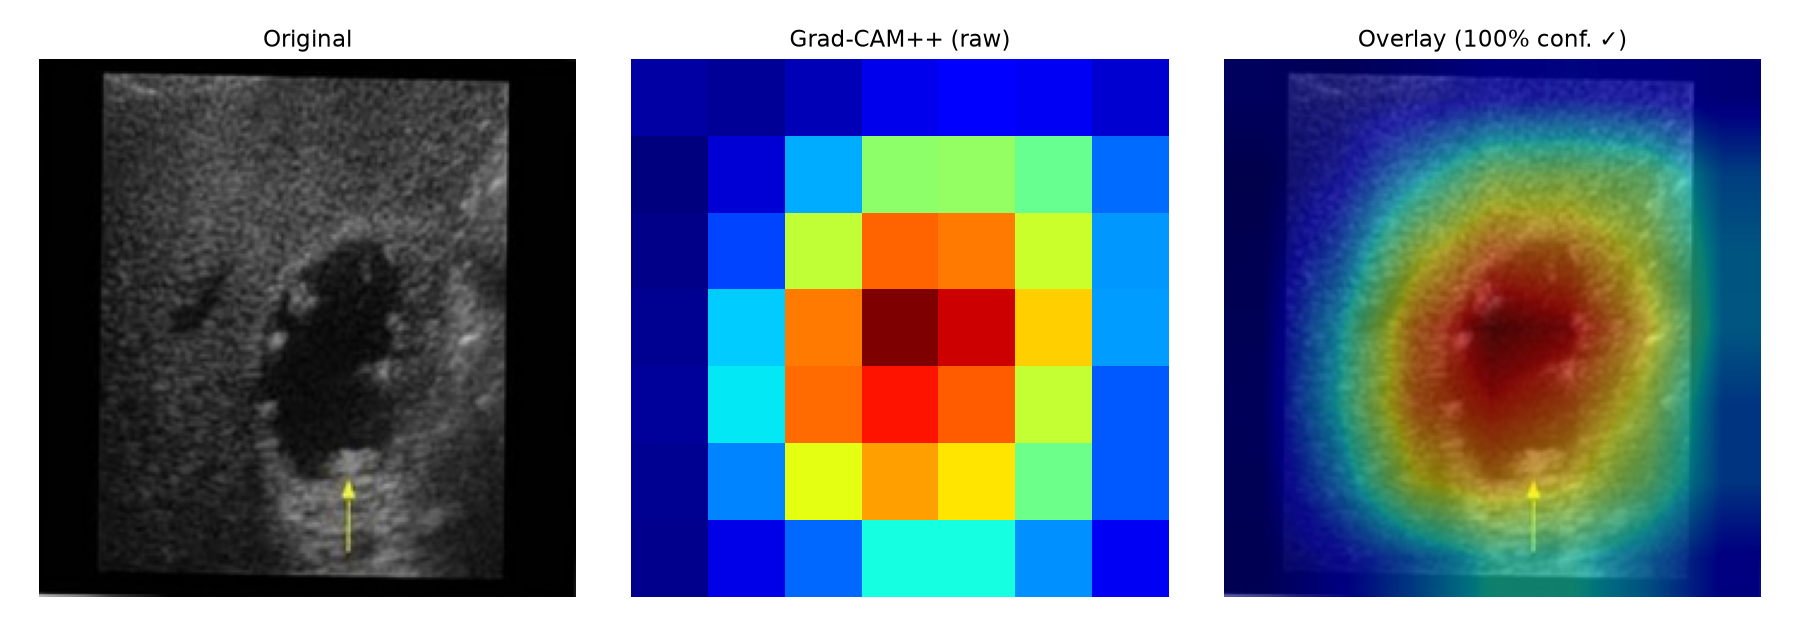
\includegraphics[width=0.48\linewidth]{figures/fig7_expanded/06_polyps_and_cholesterol_crystals_01}\\[2pt]
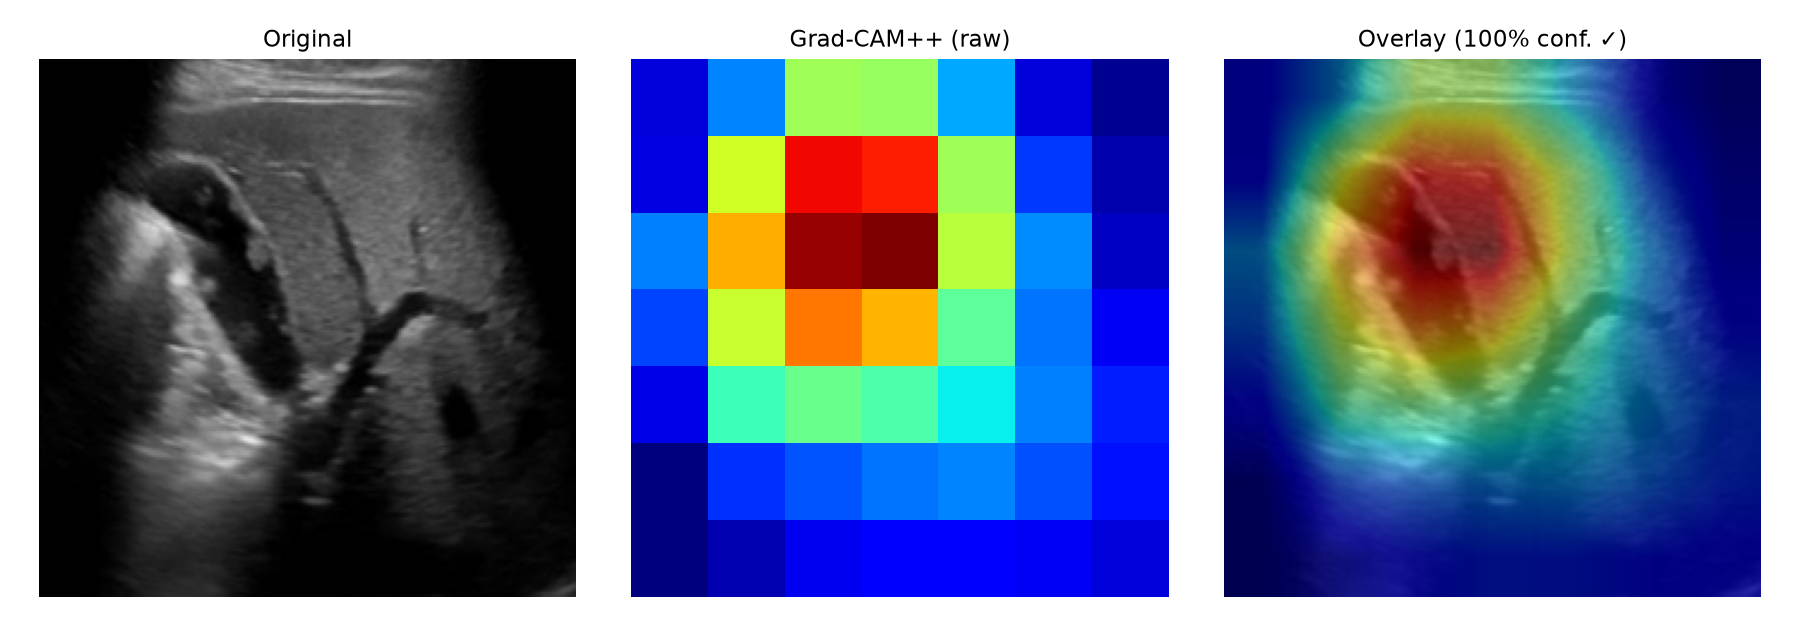
\includegraphics[width=0.48\linewidth]{figures/fig7_expanded/06_polyps_and_cholesterol_crystals_02}\hfill
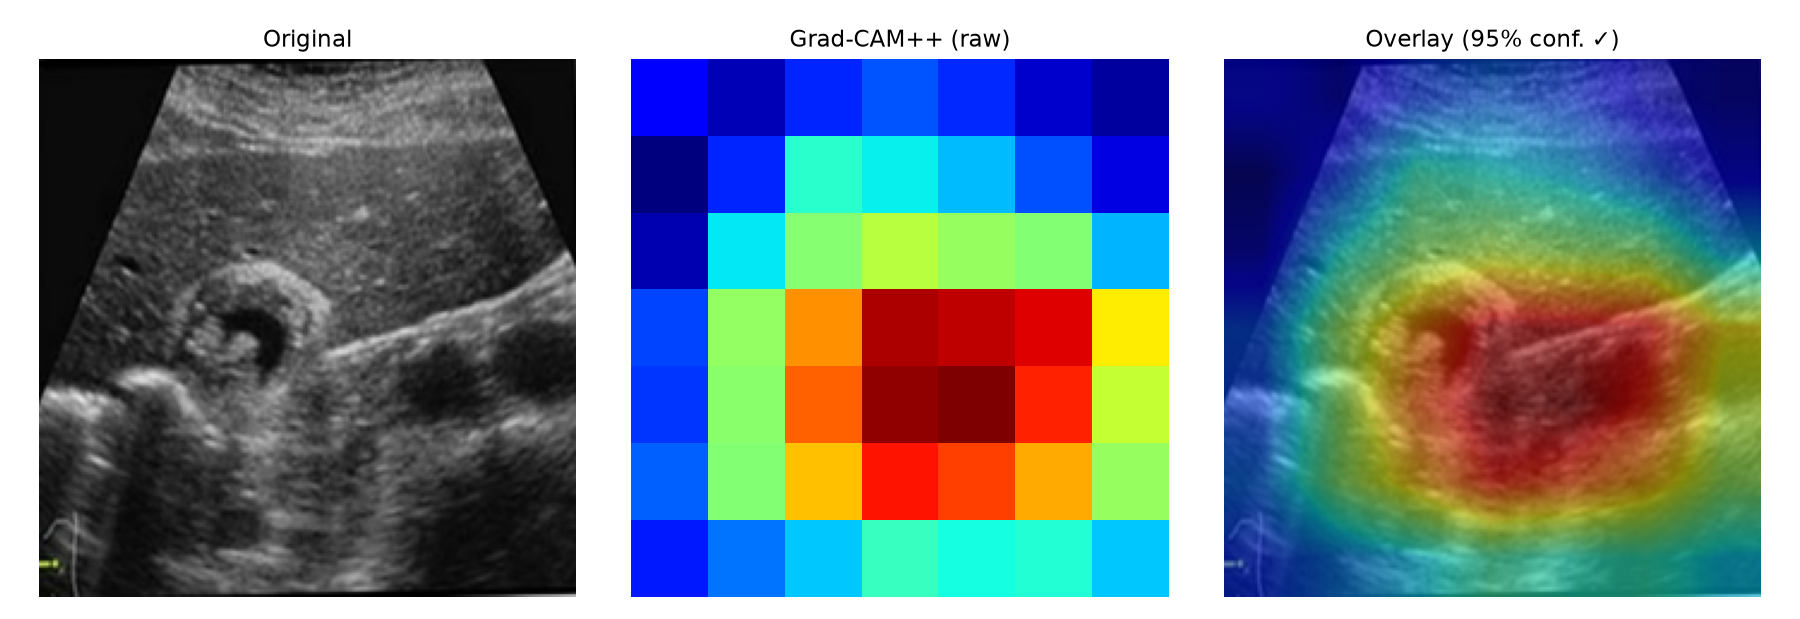
\includegraphics[width=0.48\linewidth]{figures/fig7_expanded/07_adenomyomatosis_01}\\[2pt]
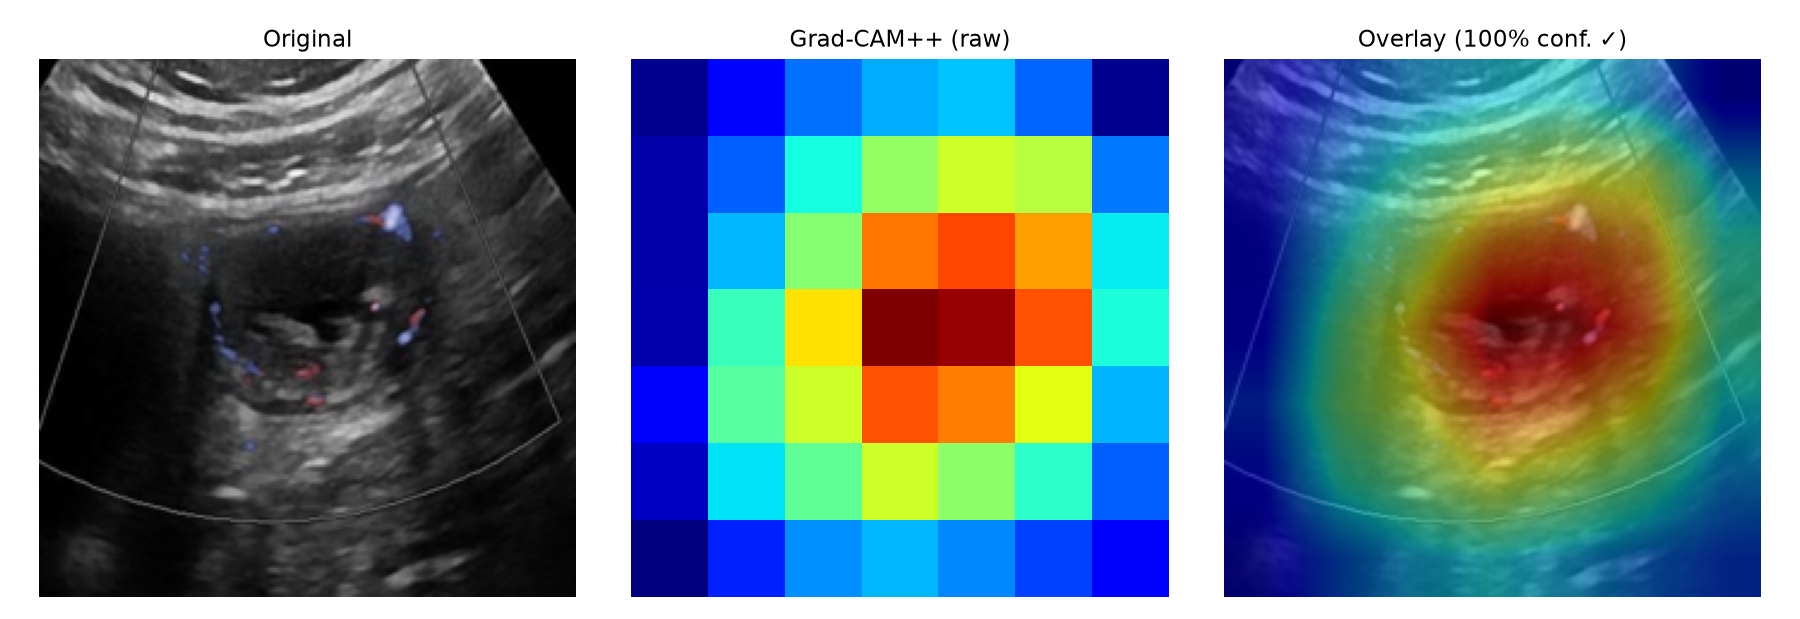
\includegraphics[width=0.48\linewidth]{figures/fig7_expanded/07_adenomyomatosis_02}\hfill
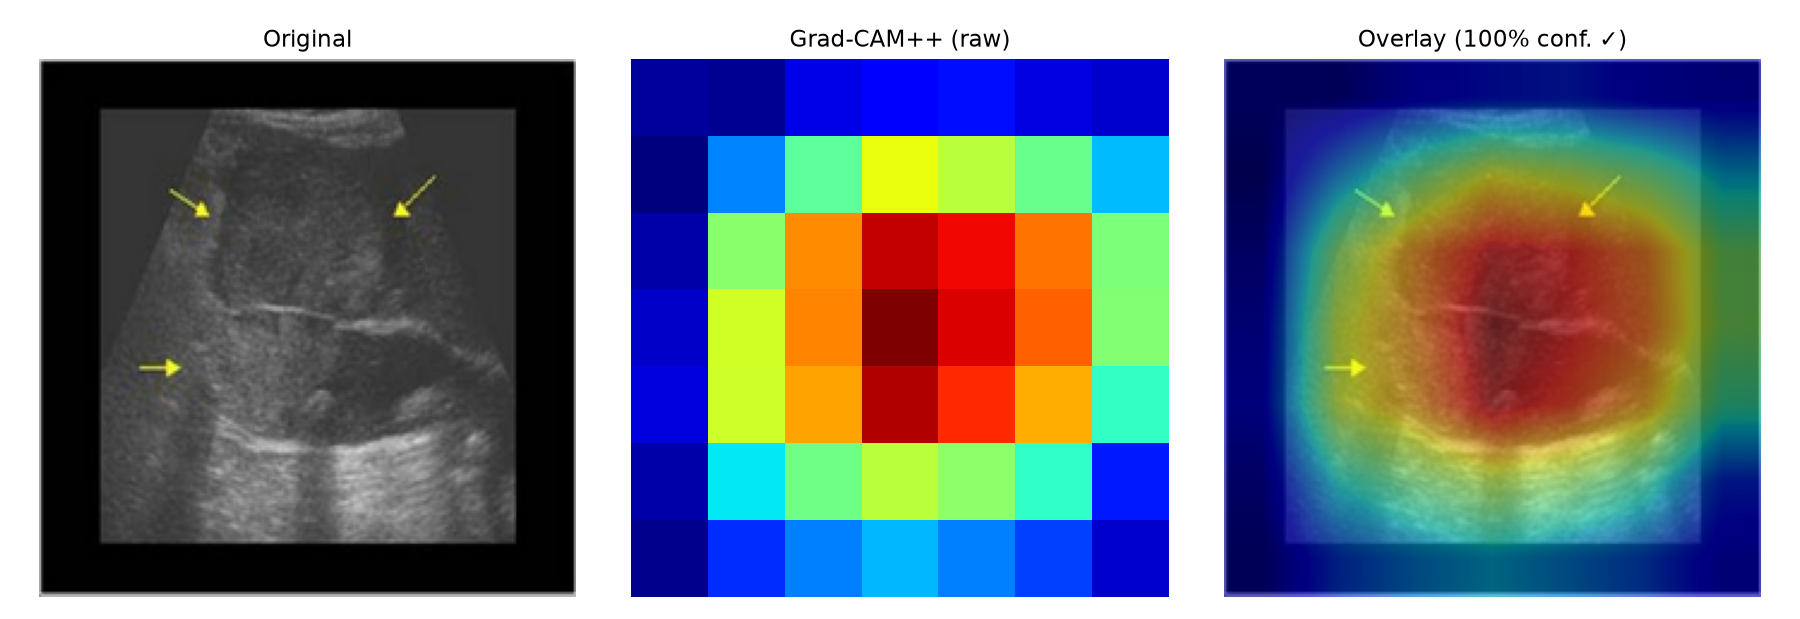
\includegraphics[width=0.48\linewidth]{figures/fig7_expanded/08_carcinoma_01}\\[2pt]
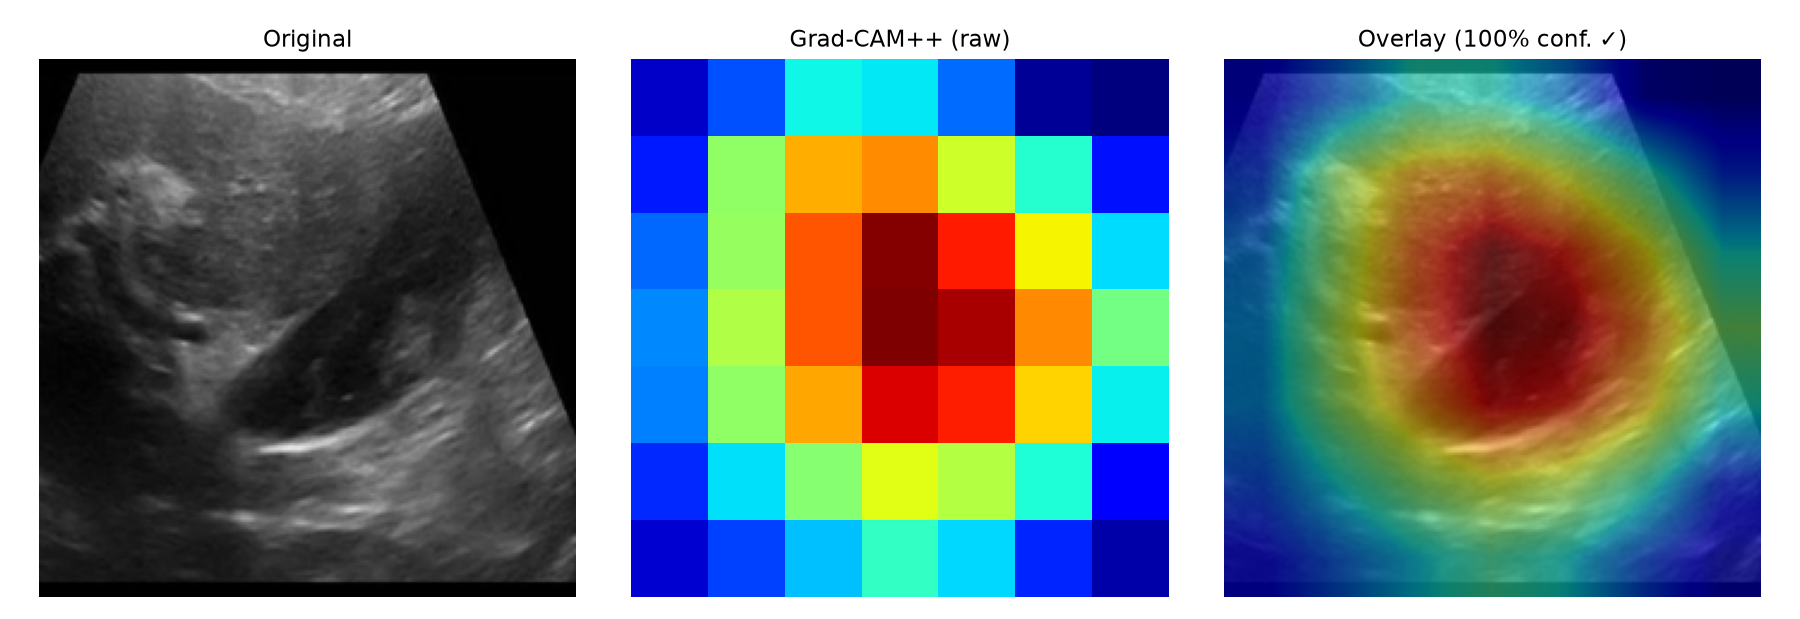
\includegraphics[width=0.48\linewidth]{figures/fig7_expanded/08_carcinoma_02}\hfill
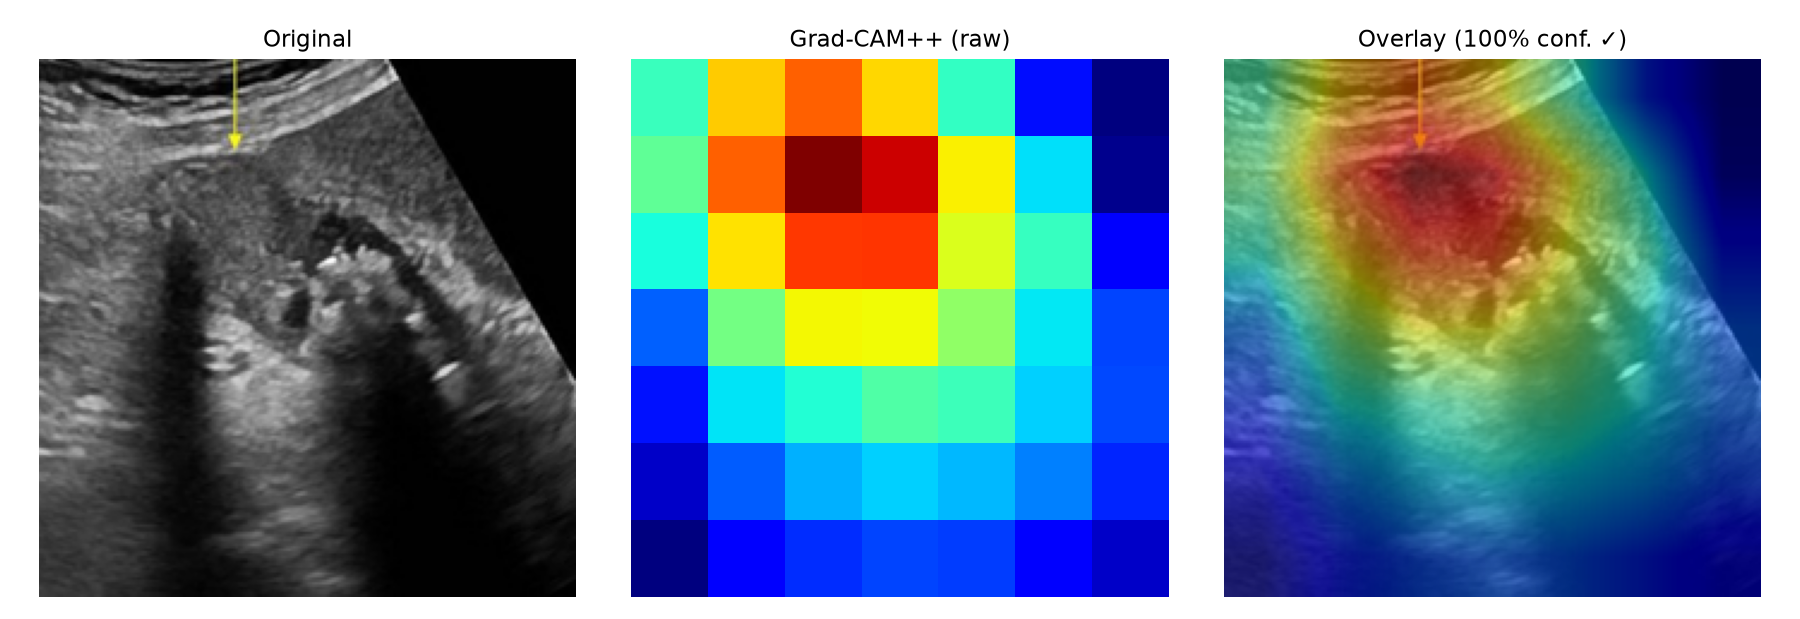
\includegraphics[width=0.48\linewidth]{figures/fig7_expanded/08_carcinoma_03}\\[2pt]
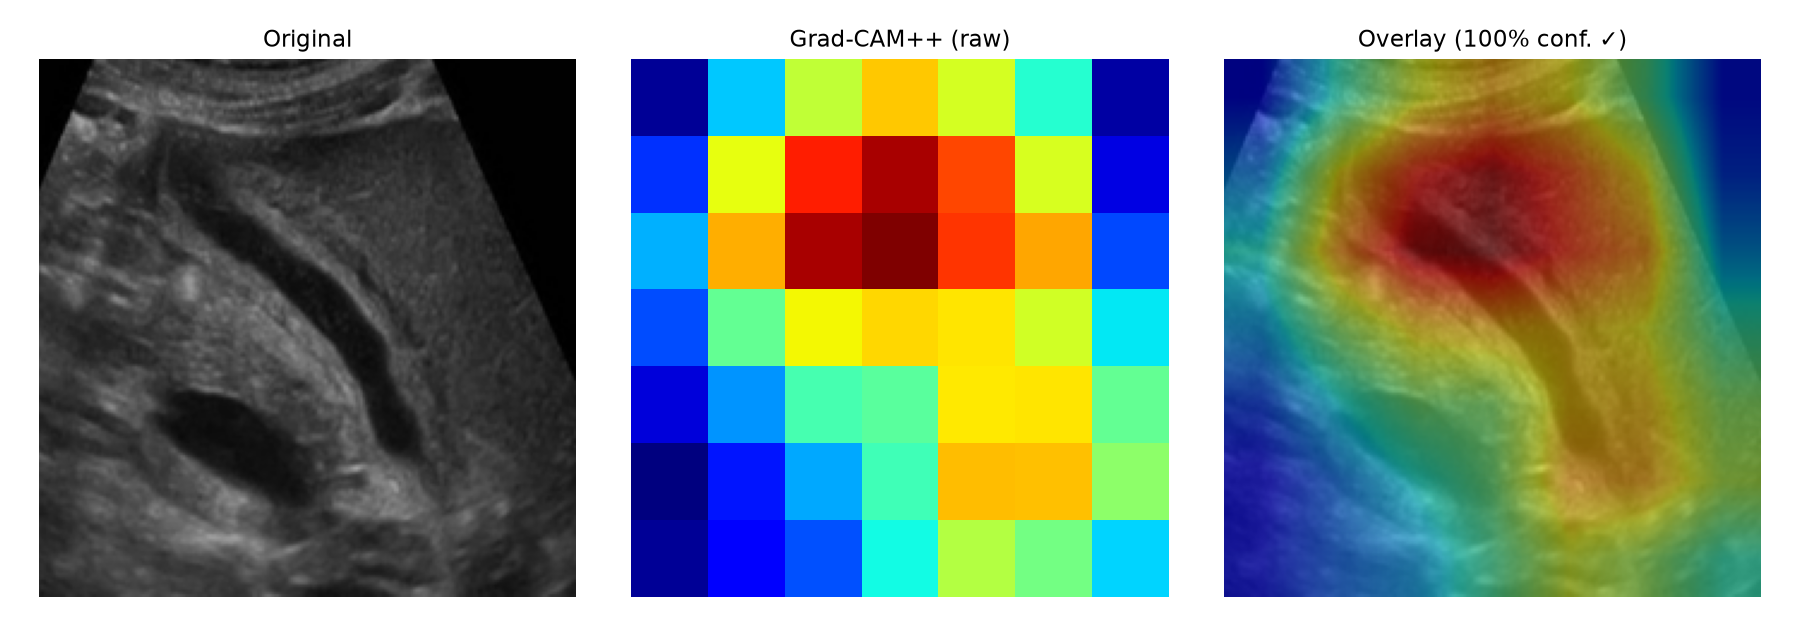
\includegraphics[width=0.48\linewidth]{figures/fig7_expanded/09_various_causes_of_gallbladder_wall_thickening_01}\hfill
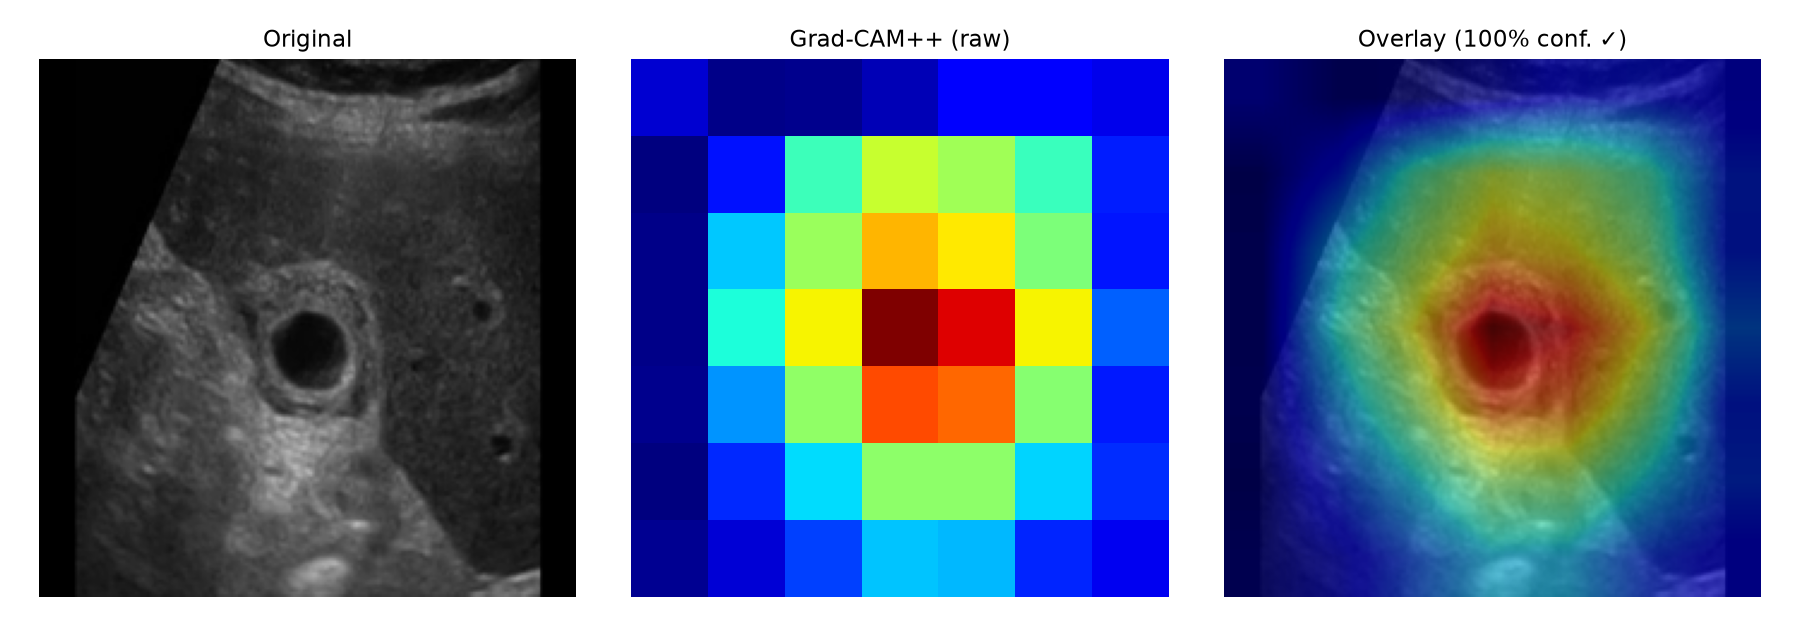
\includegraphics[width=0.48\linewidth]{figures/fig7_expanded/09_various_causes_of_gallbladder_wall_thickening_02}
\caption{Continued from Fig.~\ref{fig:8}: the remaining representative images for Perforation, Polyps \& Cholesterol Crystals, Adenomyomatosis, Carcinoma (three samples, the largest class), and Wall Thickening. Together, Figs.~\ref{fig:8}--\ref{fig:8b} cover all nine classes with 2--3 independent samples each (20 images total), confirming the heatmap patterns described above generalise across images within each class rather than reflecting one cherry-picked example.}
\label{fig:8b}
\end{figure*}

\textit{XAI Finding (4):} For Carcinoma, Grad-CAM++ and Score-CAM produce sharper, more localised wall-region attention than standard Grad-CAM. This is consistent with the expected discriminative feature for malignancy (focal wall irregularity and thickening) and makes Grad-CAM++ a strong candidate for subsequent clinician validation on this class, given its high cross-training consistency (Section~\ref{sec:results}.3) alongside competitive faithfulness (Section~\ref{sec:results}.4); this is not, absent clinician ROI validation and given Grad-CAM's comparable faithfulness score, a claim that Grad-CAM++ is the preferred visualisation method for malignancy detection in general.

\textit{XAI Finding (5):} Quantitatively, the mean cosine consistency $O_r^c$ between the primary and replicate-model Grad-CAM heatmaps across all classes and replicates is \textbf{0.769} (72 stratified validation images $\times$ 3 replicates, Section~\ref{sec:methods}.3), with wide variance across replicates (0.898, 0.629, 0.781). Grad-CAM++ and Score-CAM are both far higher and far more stable (macro mean 0.944 and 0.937 respectively). This indicates those two methods' explanations are the most consistent property of the learned decision boundary under the cross-training-replicate design of Section~\ref{sec:methods}.3---in which the replicate models are trained on disjoint subsets of the corrected training set, so the measured consistency reflects robustness to combined re-initialisation and moderate class-distribution shift, not isolated stochastic-seed variance on identical training data (Section~\ref{sec:limitations}).

\begin{table*}[!ht]
\centering
\caption{Cosine-Consistency Scores $O_r^c$ per XAI Method, Primary Model vs. Each of Three Replicates, over a Stratified 72-Image Evaluation Set (8/class~$\times$~9 classes, seed~=~42). Threshold $\theta=0.70$ flags divergent cases; best macro mean in bold. Eigen-CAM's low score reflects a mismatch between a class-agnostic method and this class-conditional metric (see note below the table), not a reliability finding comparable to the other four methods.}
\label{tbl:5}
\begin{tabular}{lccccc}
\toprule
Method & $R_1$ $O_1^c$ & $R_2$ $O_2^c$ & $R_3$ $O_3^c$ & Macro Mean~$\pm$~Std & Bootstrap 95\% CI \\
\midrule
Grad-CAM & 0.898 & 0.629 & 0.781 & 0.769~$\pm$~0.314 & $[0.735,\,0.803]$ \\
Grad-CAM++ & 0.948 & 0.935 & 0.948 & \textbf{0.944~$\pm$~0.044} & $[0.935,\,0.950]$ \\
Saliency Map & 0.686 & 0.669 & 0.689 & 0.681~$\pm$~0.037 & $[0.675,\,0.687]$ \\
Eigen-CAM & 0.280 & 0.227 & 0.220 & 0.242~$\pm$~0.343 & $[0.174,\,0.314]$ \\
Score-CAM & 0.939 & 0.934 & 0.937 & 0.937~$\pm$~0.051 & $[0.929,\,0.944]$ \\
\bottomrule
\end{tabular}

\vspace{2pt}
\raggedright\footnotesize Computed between the primary model and each of three independently trained replicate models (Section~\ref{sec:methods}.3) over the same stratified 72-image set for every method. Bootstrap 95\% CIs use 2,000 image-level resamples (with replacement) of the macro mean, added in response to a review noting no XAI table in the paper carried a confidence interval; note that Grad-CAM++'s and Score-CAM's intervals do not overlap Grad-CAM's, Saliency's, or Eigen-CAM's, supporting the claim that their consistency advantage is not merely noise at this sample size, while Grad-CAM++'s and Score-CAM's own intervals substantially overlap each other. This quantifies explanation reproducibility only; it is not a measure of diagnostic or localization correctness, which requires clinician-annotated regions of interest (Section~\ref{sec:future-research}). \textit{Eigen-CAM caveat:} Eigen-CAM is class-agnostic by construction (Section~\ref{sec:methods}.3): its output does not condition on the explained class $c$ at all, so it computes the same dominant-activation map regardless of which class is being explained. The $O_r^c$ metric compares heatmaps produced \textit{for a specific class}, a criterion Eigen-CAM's design does not target. Its low score here is therefore a mismatch between a class-conditional metric and a class-agnostic method, not direct evidence that Eigen-CAM's explanations are less reliable than the other four; a fair reliability comparison for Eigen-CAM would require a class-agnostic consistency measure, which this paper does not compute.
\end{table*}

\begin{table*}[!ht]
\centering
\caption{Cosine-Consistency Mean $\bar{O}^c$ per Class, Compared Across All Five XAI Methods (Averaged over $R_1$, $R_2$, $R_3$; Stratified 72-Image Evaluation Set, seed~=~42). Best method per class in bold.}
\label{tbl:6}
\begin{tabular}{lccccc}
\toprule
Class & Grad-CAM & Grad-CAM++ & Saliency Map & Eigen-CAM & Score-CAM \\
\midrule
Gallstones (GS) & 0.595 & \textbf{0.932} & 0.651 & 0.271 & 0.928 \\
Abdomen \& Retroperitoneum (ART) & 0.850 & 0.941 & 0.702 & 0.255 & \textbf{0.934} \\
Cholecystitis (CHOL) & 0.860 & \textbf{0.943} & 0.670 & 0.333 & 0.943 \\
Membranous/Gangrenous Cholecystitis (MGC) & 0.727 & \textbf{0.959} & 0.681 & 0.073 & 0.931 \\
Perforation (PERF) & 0.749 & \textbf{0.941} & 0.678 & 0.379 & 0.932 \\
Polyps \& Cholesterol Crystals (PCC) & 0.873 & \textbf{0.959} & 0.697 & 0.526 & 0.956 \\
Adenomyomatosis (ADNM) & 0.895 & 0.939 & 0.688 & 0.085 & \textbf{0.943} \\
Carcinoma (CARC) & 0.742 & \textbf{0.917} & 0.686 & 0.192 & 0.911 \\
Wall Thickening (WT) & 0.630 & 0.962 & 0.680 & 0.066 & \textbf{0.953} \\
\midrule
\textbf{Macro Mean} & 0.769 & \textbf{0.944} & 0.681 & 0.242 & 0.937 \\
\bottomrule
\end{tabular}

\vspace{2pt}
\raggedright\footnotesize Grad-CAM++ achieves the highest macro-mean consistency overall ($\bar{O}^c=0.944$) and wins six of nine classes; Score-CAM is a close second overall ($\bar{O}^c=0.937$) and wins the remaining three. Both anchor their weighting to the target class's evidence---Grad-CAM++ via second-order gradient weighting, Score-CAM via each channel's actual effect on the softmax score---avoiding the gradient saturation/noise that can affect plain Grad-CAM, which is far more volatile ($\bar{O}^c=0.769\pm0.314$) and collapses for Gallstones and Wall Thickening (0.595, 0.630); Saliency Maps' finer pixel-space granularity similarly makes small per-model differences contribute disproportionately to cosine divergence ($\bar{O}^c=0.681$). Neither pattern should be read as evidence these two methods' explanations are less clinically meaningful, only less reproducible across retraining under this design. Eigen-CAM's near-zero score ($\bar{O}^c=0.242$, falling below 0.10 for three classes) is excluded from this ranking-by-magnitude reading entirely: as Table~\ref{tbl:5}'s note explains, Eigen-CAM is class-agnostic and this metric is class-conditional, so its low score reflects that mismatch rather than a genuine reliability deficit comparable to the other four methods.
\end{table*}

\begin{figure*}[!ht]
\centering
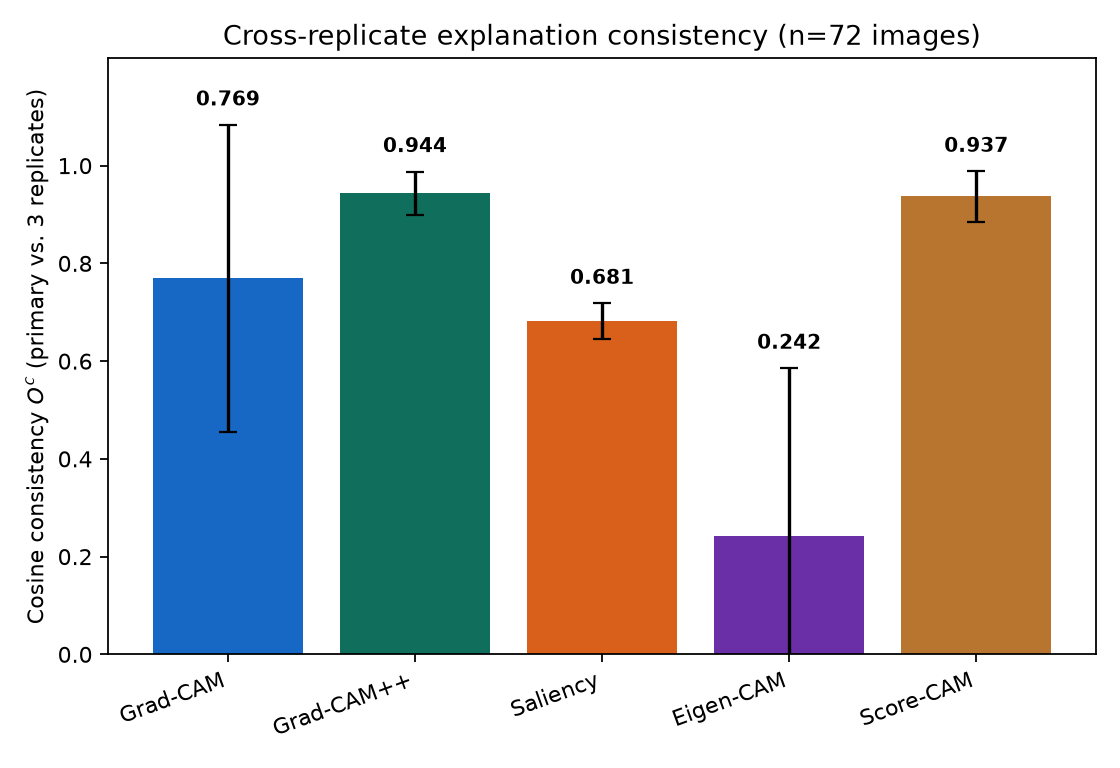
\includegraphics[width=0.55\textwidth]{figures/consistency.png}
\caption{Visual companion to Table~\ref{tbl:5}: macro cosine-consistency mean~$\pm$~std for each of the five XAI methods (72-image stratified set, three replicates). Grad-CAM++ and Score-CAM cluster tightly near 0.94; Grad-CAM shows the widest error bar of the three CAM-family methods; Eigen-CAM is both lowest and most volatile.}
\label{fig:9}
\end{figure*}

Table~\ref{tbl:6} reveals three consistent patterns. First, Grad-CAM++ and Score-CAM stay above $\theta=0.70$ for all nine classes, while plain Grad-CAM drops below threshold for two classes it would otherwise be expected to handle well (Gallstones 0.595, Wall Thickening 0.630), suggesting Grad-CAM's coarser, unweighted feature-map averaging, rather than class difficulty, is the limiting factor. Second, Eigen-CAM collapses almost completely for Membranous/Gangrenous Cholecystitis, Adenomyomatosis, and Wall Thickening ($\bar{O}^c=0.073$, $0.085$, $0.066$), consistent with these three classes having the most diffuse, least focal discriminative regions (Section~\ref{sec:results}.3), which leaves Eigen-CAM's unsupervised principal component with the least consistent direction to lock onto across training subsets. Third, Grad-CAM's per-replicate breakdown (Table~\ref{tbl:5}: 0.898, 0.629, 0.781) shows replicate $R_2$, trained on the smallest subset (2,089~images), diverging most from the primary model, whereas Grad-CAM++ and Score-CAM stay tightly clustered regardless of subset size: the two best methods are also the most robust to training-data volume.

\subsection{Quantitative reliability battery}

\textbf{Faithfulness.} Cross-replicate consistency (Section~\ref{sec:results}.3) establishes that explanations are reproducible, but not that they are \textit{faithful}, in the sense that the highlighted pixels are the ones the model actually relies on. Faithfulness is tested directly with deletion and insertion curves \cite{ref14}: starting from each validation image, the most-attributed pixels are progressively replaced with a blurred baseline (deletion, where a faithful map makes the predicted-class probability fall fast, so \textit{lower} area-under-curve is better), and separately restored onto a blurred baseline (insertion, where a faithful map makes probability rise fast, so \textit{higher} AUC is better). Each method is compared against a random pixel-ordering control on the same 144 stratified images (20 removal/insertion steps). This test is run for the three methods that anchor their weighting to the target class's evidence in feature-map space (Grad-CAM, Grad-CAM++, Score-CAM); Eigen-CAM is excluded because it is class-agnostic and so has no class-specific attribution ordering for this test to remove or restore, and Saliency Maps are excluded because they attribute in raw pixel space rather than the feature-map space the deletion/insertion baseline masking here assumes, making a direct three-way comparison with the CAM-family methods not straightforwardly meaningful.

\begin{table}[!ht]
\centering
\caption{Deletion / Insertion Faithfulness (144 stratified validation images, 20 steps). Lower deletion AUC and higher insertion AUC are better; the gap (insertion~$-$~deletion) is a single faithfulness score. All three CAM methods beat the random control by a wide margin. Eigen-CAM and Saliency Maps are not included; see the exclusion rationale above.}
\label{tbl:7}
\begin{tabular}{lcccc}
\toprule
Method & Deletion AUC~$\downarrow$ & Insertion AUC~$\uparrow$ & Gap~$\uparrow$ & Gap Bootstrap 95\% CI \\
\midrule
Grad-CAM & 0.307 & \textbf{0.787} & \textbf{0.480} & $[0.437,\,0.518]$ \\
Grad-CAM++ & \textbf{0.312} & 0.785 & 0.473 & $[0.430,\,0.515]$ \\
Score-CAM & 0.323 & 0.778 & 0.456 & $[0.413,\,0.498]$ \\
Random control & 0.610 & 0.597 & $-0.013$ & $[-0.024,\,-0.004]$ \\
\bottomrule
\end{tabular}

\vspace{2pt}
\raggedright\footnotesize Gap bootstrap 95\% CIs use 2,000 image-level resamples (with replacement), added in response to a review noting the close three-way faithfulness ranking (0.480 vs.\ 0.473 vs.\ 0.456) had no interval showing whether it was distinguishable from noise: all three CAM methods' intervals overlap substantially, confirming the ranking should not be over-interpreted, exactly as XAI Finding~(6) already states qualitatively. The random control's interval excludes zero but remains far below all three CAM methods, the expected null result.
\end{table}

\begin{figure*}[!ht]
\centering
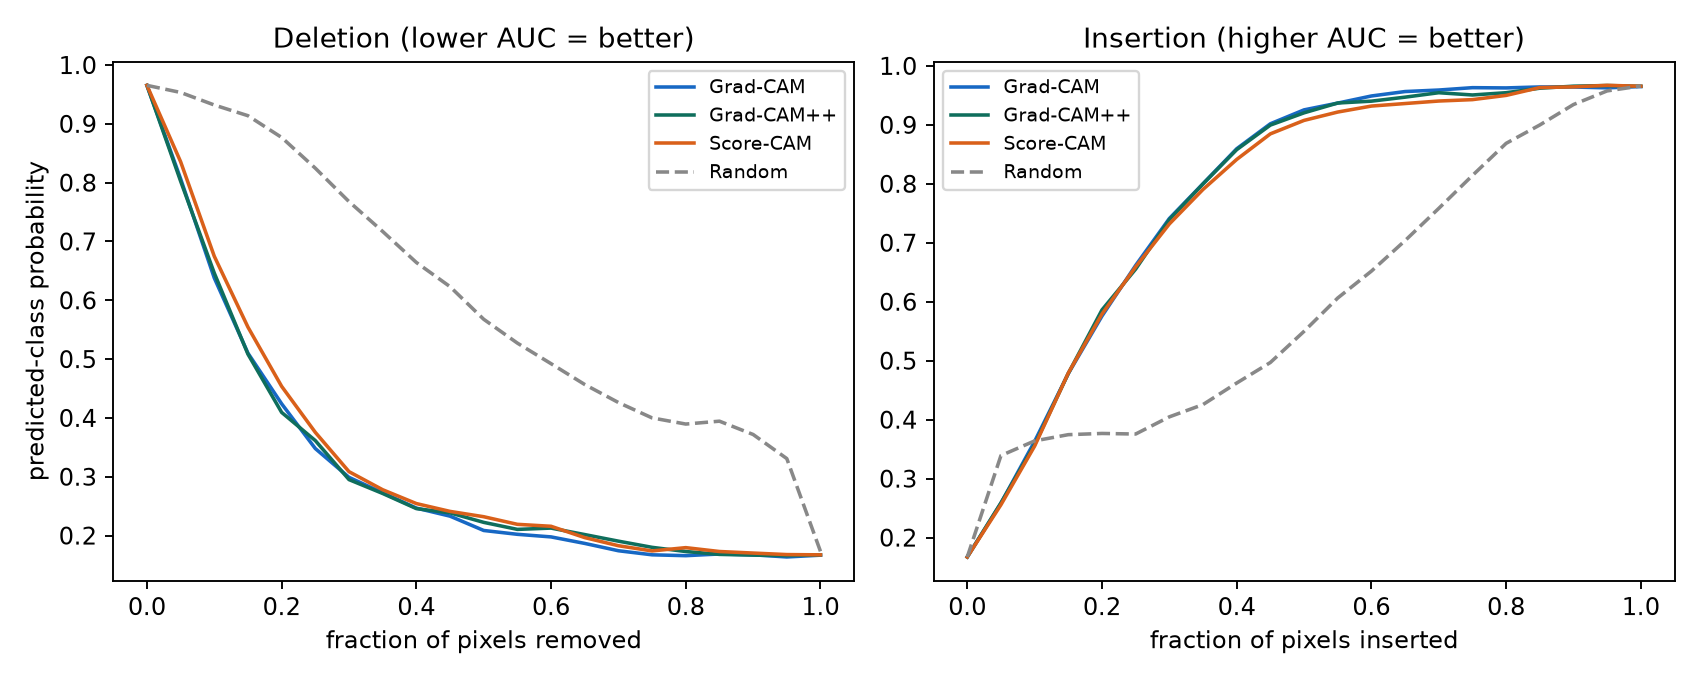
\includegraphics[width=0.7\textwidth]{figures/faithfulness.png}
\caption{Mean deletion (left) and insertion (right) curves. All three CAM methods sit far below the random control under deletion and far above it under insertion, confirming their heatmaps are faithful to the model's decision rather than merely plausible. The random control's near-zero gap (Table~\ref{tbl:7}) is the expected null result.}
\label{fig:10}
\end{figure*}

\textit{XAI Finding (6):} All three CAM-family methods are faithful by the deletion/insertion criterion, each beating the random control by a wide margin (gap 0.46--0.48 vs. $-0.013$). The three-way ranking among them (Grad-CAM 0.480, Grad-CAM++ 0.473, Score-CAM 0.456) is too close to over-interpret. This quantitative result, not the visual plausibility of the Section~\ref{sec:results}.2 failure-case heatmaps, is what licenses trusting the explanations.

\textbf{Stability.} A reliable explanation should not shift substantially under image perturbations that are intended to be diagnostically minor. Three candidate transforms are applied to 216 stratified validation images: a $\times1.15$ brightness shift, a 10-pixel diagonal translation (heatmap realigned before comparison), and additive Gaussian noise ($\sigma=0.03$). As the prediction-retention column of Table~\ref{tbl:8} below shows, though, not all three actually leave the classifier's own prediction unchanged; only brightness does so reliably. For each transform, Grad-CAM++ is recomputed for the originally predicted class, and agreement with the unperturbed heatmap is measured via SSIM, Pearson correlation, and top-10\% pixel overlap (IoU), together with the fraction of images whose predicted class is unchanged. Because prediction changes and explanation changes are conflated whenever a transform is not prediction-preserving, the headline SSIM/Pearson/IoU numbers below should be read as agreement over all 216 images regardless of whether the prediction held; XAI Finding~(7) separates the two effects explicitly for the noise transform, where the distinction matters most.

\begin{table}[!ht]
\centering
\caption{Grad-CAM++ Explanation Stability Under Candidate Minor-Perturbation Transforms (216 stratified validation images). ``Pred. kept'' shows only brightness is reliably prediction-preserving; translation and noise are not.}
\label{tbl:8}
\begin{tabular}{lcccc}
\toprule
Transform & SSIM (95\% CI) & Pearson & Top-10\% IoU & Pred. kept \\
\midrule
Brightness ($\times1.15$) & \textbf{0.995} $[0.994,0.995]$ & \textbf{0.998} & \textbf{0.907} & \textbf{98.6\%} \\
Translation (10~px) & 0.848 $[0.845,0.852]$ & 0.931 & 0.681 & 93.5\% \\
Gaussian noise ($\sigma=0.03$) & 0.931 $[0.926,0.936]$ & 0.950 & 0.652 & 70.8\% \\
\bottomrule
\end{tabular}

\vspace{2pt}
\raggedright\footnotesize SSIM 95\% CIs use 2,000 image-level bootstrap resamples, added in response to a review noting no XAI table carried a confidence interval; all three transforms' SSIM intervals are narrow and non-overlapping, so the brightness/translation/noise ranking in this column is well-supported at this sample size. Pearson and top-10\% IoU bootstrap 95\% CIs (also computed, narrow in every case, e.g.\ Pearson brightness $[0.997,\,0.998]$, translation $[0.923,\,0.937]$, noise $[0.942,\,0.957]$; top-10\% IoU brightness $[0.896,\,0.917]$, translation $[0.659,\,0.704]$, noise $[0.627,\,0.676]$) are omitted from the table for space but available in \texttt{outputs/phase0/stability.json}.
\end{table}

\begin{figure*}[!ht]
\centering
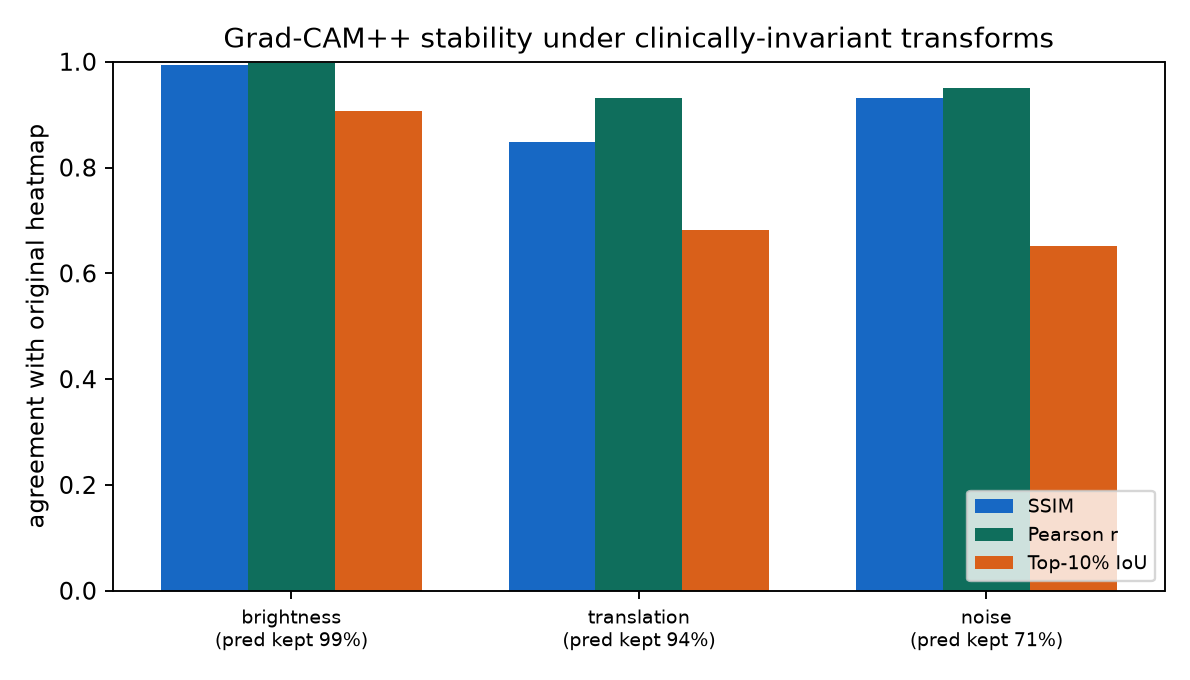
\includegraphics[width=0.6\textwidth]{figures/stability.png}
\caption{Grad-CAM++ explanation stability under the three transforms. Brightness is near-perfectly stable on every axis; translation and noise diverge---translation disturbs the heatmap's pixel-level structure (lowest SSIM) more than noise does, while noise disturbs the model's actual prediction (lowest prediction-kept rate) far more than translation does.}
\label{fig:11}
\end{figure*}

\textit{XAI Finding (7):} Grad-CAM++ is highly stable under brightness change (SSIM~0.995, prediction kept 98.6\%), but translation and noise disrupt different things. Translation degrades the heatmap most (SSIM~0.848) while leaving the prediction largely intact (93.5\% kept). Noise leaves the heatmap comparatively more intact (SSIM~0.931) but flips the predicted class nearly 30\% of the time (70.8\% kept). Since noise changes what the model outputs, not just how it explains that output, classifier-level noise robustness---not explanation robustness---is the more urgent target for future training.

\textbf{Model-parameter randomization sanity check.} A trustworthy saliency method must depend on the model's learned weights, yet some popular methods notoriously do not \cite{ref13}. Following the Adebayo et~al. protocol, ResNet-50's parameters are cascade-randomized from the output layer back toward the input (fc~$\rightarrow$~layer4~$\rightarrow$~$\dots$~$\rightarrow$~conv1), Grad-CAM++ is recomputed for the same explained class at each stage, and similarity to the fully-trained-model heatmap is measured (108 images). As Fig.~\ref{fig:12} shows, similarity is highest when only \texttt{fc} is randomized ($|\rho|=0.95$), which is expected since Grad-CAM++ taps \texttt{layer4} and \texttt{fc} lies downstream of that tap. It then drops sharply as soon as \texttt{layer4} itself is randomized ($|\rho|=0.52$), keeps falling through \texttt{layer3} and \texttt{layer2}, and reaches its minimum at \texttt{layer1} ($|\rho|=0.20$), with a modest uptick at \texttt{conv1} ($|\rho|=0.33$) that stays far below the trained-model value. The heatmap therefore genuinely depends on the learned convolutional features rather than acting as an input-edge detector, and the method passes the sanity check.

\begin{figure*}[!ht]
\centering
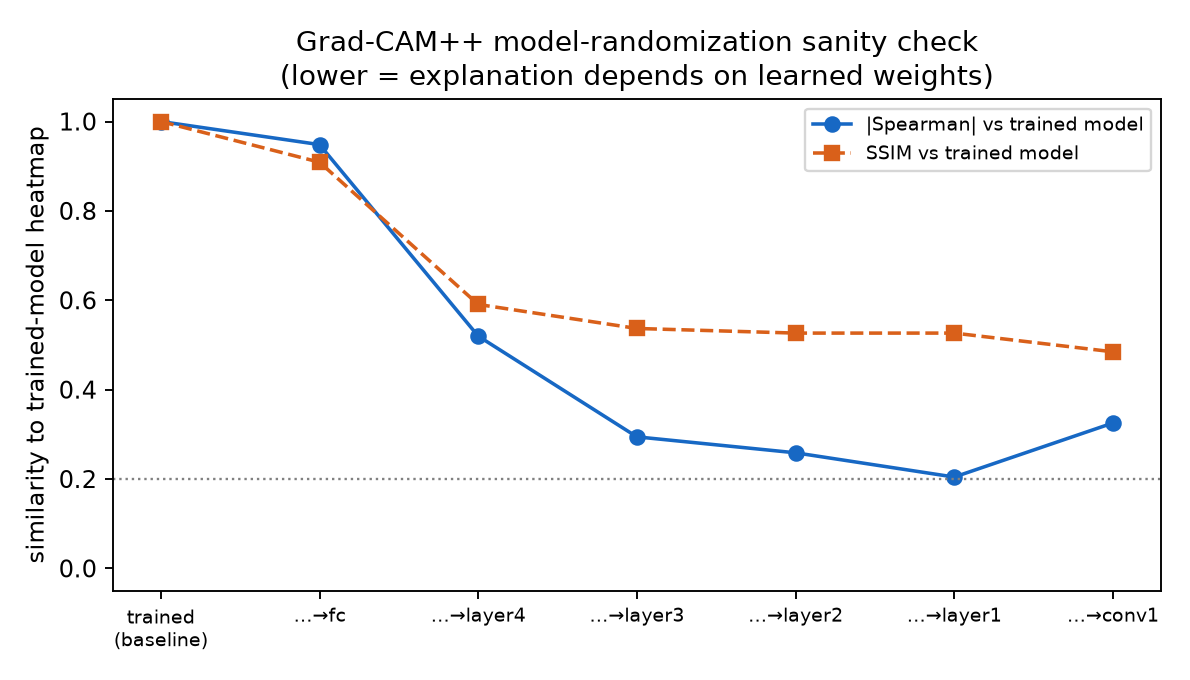
\includegraphics[width=0.6\textwidth]{figures/sanity_checks.png}
\caption{Model-randomization sanity check. Grad-CAM++ heatmap similarity to the trained model (absolute Spearman correlation and SSIM) drops sharply once \texttt{layer4}---the Grad-CAM++ tap point---is randomized and continues declining through the remaining convolutional stages, confirming the explanation reflects learned weights rather than acting as an input-edge detector.}
\label{fig:12}
\end{figure*}

\textbf{Probability calibration.} Unlike the faithfulness, stability, sanity-check, and shortcut-audit results above, calibration is a property of the underlying classifier's confidence output, not of any XAI explanation. It is reported alongside the explanation-reliability battery because both jointly determine whether the model's overall output, prediction, confidence, and explanation together, can be trusted, not because calibration is itself a measure of explanation quality. Section~\ref{sec:results}.2 noted that the model's raw softmax confidence separates correct from incorrect predictions but is not a calibrated probability; that observation is now quantified and corrected. A single temperature parameter \cite{ref42} is fit on a stratified calibration half of the validation set (1,594 images) and evaluated on the held-out half (1,599 images, accuracy~0.9318). Temperature scaling ($T=1.468$) reduces Expected Calibration Error from 0.034 to 0.009 and the Brier score from 0.109 to 0.106, without altering discrimination, since accuracy is unchanged by construction. Fig.~\ref{fig:13} shows the model is mildly over-confident before scaling, with its reliability curve sitting slightly below the diagonal at high confidence, and closely calibrated afterward.

\begin{figure}[!ht]
\centering
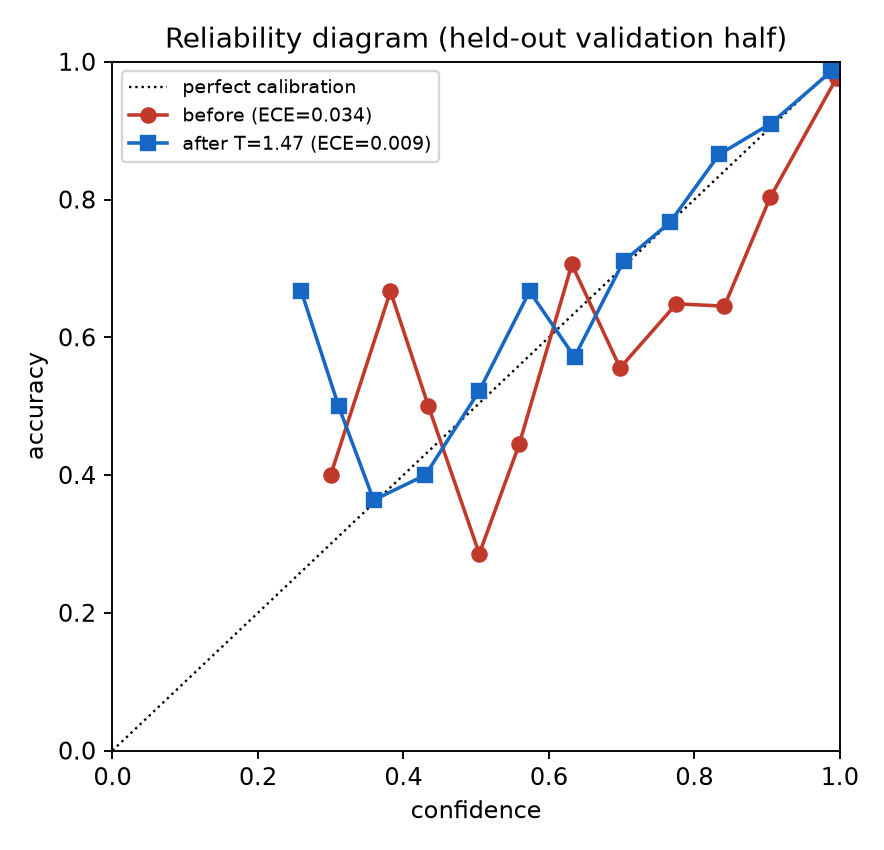
\includegraphics[width=0.85\linewidth]{figures/calibration.png}
\caption{Reliability diagram on the held-out validation half. Temperature scaling ($T=1.468$) moves the confidence--accuracy curve toward the diagonal, cutting ECE by 73\% (0.034~$\rightarrow$~0.009).}
\label{fig:13}
\end{figure}

\textbf{Shortcut-learning audit.} Finally, this section tests one narrow, specific shortcut hypothesis: whether the model exploits non-clinical cues at the image margin (burned-in text, calipers, borders) rather than central image content \cite{ref40}, \cite{ref41}, via two measurements on 216 stratified images (Fig.~\ref{fig:14}). Cropping away the outer 12\% margin and resizing back changes accuracy substantially, from 0.9305 to 0.7122 ($-0.2183$) and macro-F1 from 0.9303 to 0.7039, while only 21.8\% ($\pm$~4.9\%) of Grad-CAM++ attribution mass falls in that margin ring, even though the ring occupies 41.0\% of the frame, markedly \textit{under}-weighted relative to its area. These two measurements point in different directions and are both reported honestly. Attribution mass being under-represented in the margin region provides no strong attribution-level evidence of margin-shortcut reliance, though attribution is not exhaustive proof of causal non-reliance. The much larger accuracy drop is not, on its own, evidence of margin-shortcut reliance either, and the crop-ablation result should be interpreted cautiously: a 12\% crop removes genuine peripheral gallbladder and adjacent-organ anatomy along with any border artefact, and for a nine-class task with several visually similar classes (Section~\ref{sec:results}.2) losing that anatomy plausibly costs real discriminative signal independent of any shortcut, confounding the two possible explanations for the drop. The crop-accuracy drop is therefore treated as a robustness finding rather than clean evidence of shortcut learning, with the border-energy result treated as the actual, narrow, margin-only shortcut audit. This audit does not test for, and does not rule out, other shortcuts a classifier could in principle learn: scanner-specific artefacts, hospital- or site-correlated imaging conventions, compression artefacts, or other background cues not tied to the image margin specifically.

\begin{figure*}[!ht]
\centering
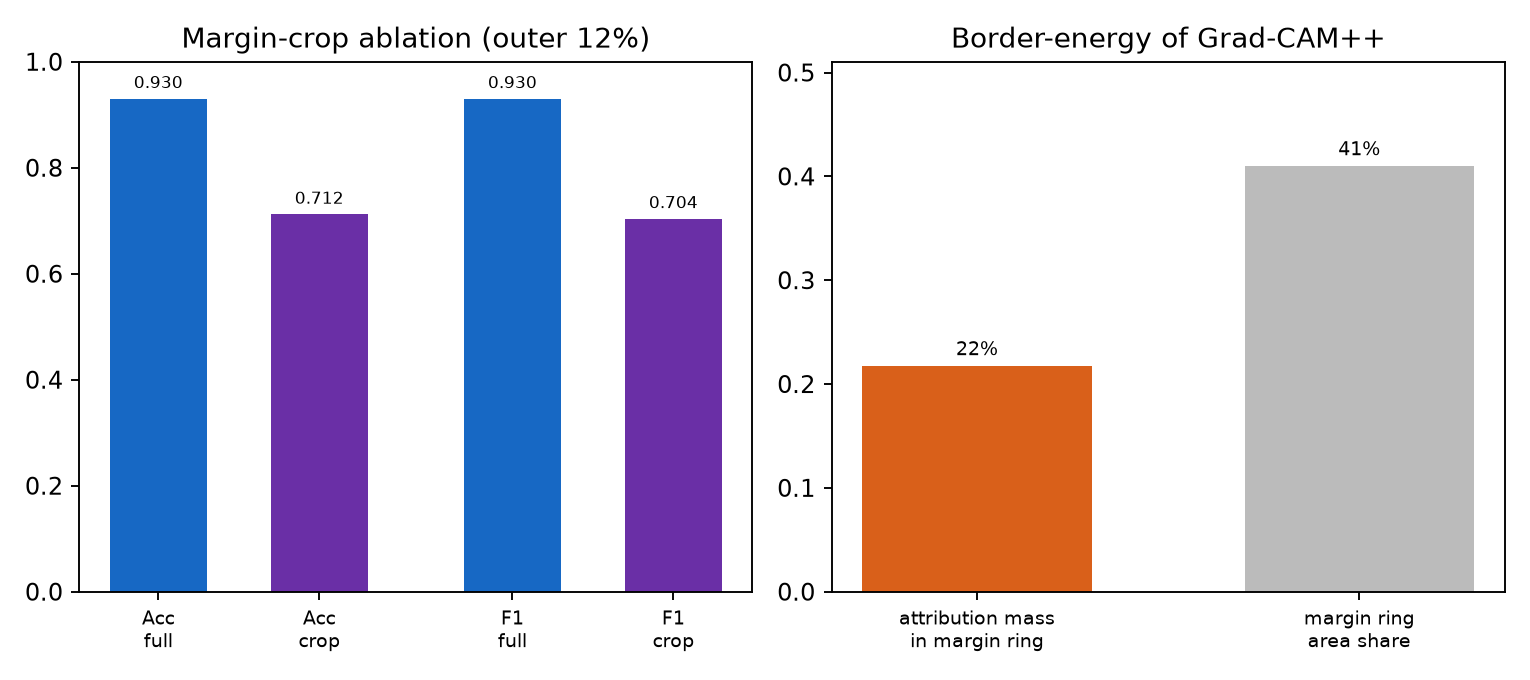
\includegraphics[width=0.65\textwidth]{figures/shortcut_audit.png}
\caption{Shortcut audit. Left: classification accuracy and macro-F1 both drop substantially under the outer-12\%-margin crop. Right: Grad-CAM++ places only 21.8\% of its attribution mass in that margin ring (which covers 41.0\% of the frame), indicating central-anatomy focus in the explanation even though the crop itself is costly to accuracy.}
\label{fig:14}
\end{figure*}

\textit{XAI Finding (8):} Attribution mass is markedly under-represented at the frame margin (21.8\% of mass in a 41.0\%-area ring), evidence against margin-shortcut reliance. The much larger crop-ablation accuracy drop (0.930~$\rightarrow$~0.712) is interpreted as genuine peripheral-anatomy dependence rather than a shortcut the border-energy measurement missed, but this is the one reliability result in the paper that is not fully clean (Section~\ref{sec:future-research}).

\subsection{Summary of key findings}

Three findings carry across Sections~\ref{sec:results}.1--4. Grad-CAM++ and Score-CAM lead on cross-replicate consistency, the reliability axis with the clearest separation between methods, but that lead does not carry over to faithfulness, where all three CAM-family methods are comparable and plain Grad-CAM numerically edges out the other two, so no method leads on every axis measured. The explanations are quantitatively faithful to the model's decision, yet heatmap plausibility alone flags neither high-confidence errors (Section~\ref{sec:results}.2) nor subtler failure modes in general, so reliability has to be measured rather than inferred from appearance. Of the reliability axes, only the shortcut audit is inconclusive, for the crop-versus-anatomy reason given in Section~\ref{sec:results}.4.

\subsection{Stage 2: cluster-aware split with a genuine held-out test set}
\label{sec:stage2}

The results above (Sections~\ref{sec:results}.1--4) come from the Stage~1 pipeline: images de-duplicated by single-orientation perceptual hashing (Section~\ref{sec:methods}.1), then split 70/30 into training and validation, with every number in this paper reported on that validation set. A subsequent, independent audit found this correction incomplete in two ways. First, 96.73\% of images share a filename-prefix ``session'' that the Stage~1 split did not keep together, so near-identical frames from the same imaging session could land on both sides of the train/validation boundary. Second, the dataset's own source publication confirms images were released after augmentation by rotation, flipping, and brightness/contrast/saturation jitter, and a rotation-aware (dihedral) hash re-check found 46\% of the corpus (4,918 of 10,692 images) has at least one cross-split duplicate that single-orientation hashing could not detect.

A Stage~2 pipeline addresses both gaps together. Every image is assigned to a duplicate cluster using an 8-orientation (dihedral) perceptual hash (1,570 clusters from the full 10,692-image corpus), and the corpus is re-split at the cluster level, 70/20/10, so no cluster crosses a train/validation/test boundary and, unlike Stage~1, a test set is held out and touched exactly once, after every other design decision (epoch budget, early-stopping criterion) is already frozen. This yields 7,470 training, 2,138 validation, and 1,084 test images. A primary model (seed~42) and three replicate models (seeds~7, 123, 2027) are trained on the identical 7,470-image training set, varying only the random seed and data-loader shuffling order---correcting the Stage~1 replicate design, in which the three replicates were trained on disjoint subsets of 2,749, 2,089, and 2,661 images respectively and therefore could not isolate seed-to-seed reproducibility from data-composition effects (Limitation~2b). Training uses up to 20 epochs with early stopping on validation macro-F1 (patience~5), rather than Stage~1's fixed 10-epoch budget.

\begin{table}[!ht]
\centering
\caption{Stage 2: Held-Out Test Performance, Cluster-Aware 70/20/10 Split (Test $n=1084$). All four models see identical training data; only the random seed varies.}
\label{tbl:stage2-test}
\begin{tabular}{lccc}
\toprule
Model & Test Accuracy & Macro-F1 & Epochs to best \\
\midrule
Primary (seed~42) & 0.7030 & 0.7039 & --- \\
Replicate (seed~7) & 0.7020 & 0.6992 & --- \\
Replicate (seed~123) & 0.7482 & 0.7486 & --- \\
Replicate (seed~2027) & 0.7491 & 0.7438 & --- \\
\midrule
\textbf{Mean~$\pm$~Std} & \textbf{0.7256~$\pm$~0.0235} & \textbf{0.7239~$\pm$~0.0221} & \\
\bottomrule
\end{tabular}
\end{table}

Table~\ref{tbl:stage2-test} reports the real, unbiased test performance this design supports: a four-model mean accuracy of 72.56\%~$\pm$~2.35\% and macro-F1 of 72.39\%~$\pm$~2.21\%, all four seeds agreeing within roughly a five-point band. This is substantially lower than the Stage~1 headline of 93.05\% accuracy, and it is the more trustworthy of the two numbers precisely because Stage~1's validation set was not fully protected from cluster-level leakage. It is also markedly higher than the 29.59\% single-run figure produced by an earlier, more aggressive session-level-only correction (Section~\ref{sec:limitations}), which re-split the existing Stage~1 train/validation files at the filename-session level without also addressing the rotation-augmented-duplicate gap or retraining with a longer schedule; that figure should be read as a lower bound from an under-specified re-split rather than the pipeline's ceiling. The Stage~2 result in Table~\ref{tbl:stage2-test} is the paper's best current estimate of what this classifier, honestly evaluated, actually achieves on nine-class gallbladder ultrasound classification.

\textit{XAI Finding (9): the null-control test for the consistency metric.} A structural concern raised against the Stage~1 consistency scores in Table~\ref{tbl:5} is that Grad-CAM-family heatmaps end in a ReLU and are then min-max normalised to $[0,1]$, so two \textit{unrelated} non-negative heatmaps of the same shape may already have high cosine similarity as a mathematical artefact, independent of anything the model has learned. Two null controls quantify this floor directly. First, cross-model consistency is measured between four \textit{untrained} ResNet-50 models (ImageNet backbone, randomly initialised nine-class head, no fine-tuning): mean cosine similarity $0.333\pm0.231$ over 240 pairwise comparisons across 40 stratified test images. Second, cosine similarity is measured between pairs of purely synthetic heatmaps with no model, image, or learning involved: $0.755\pm0.044$ for independent uniform-random $[0,1]$ maps, and $0.325\pm0.107$ for ReLU-thresholded standard-Gaussian noise, min-max normalised the same way Grad-CAM's own output is---the more representative control, since it reproduces Grad-CAM's actual non-linearity rather than assuming uniform noise. Against this pair of floors ($0.33$ untrained-model, $0.33$ ReLU-Gaussian-synthetic), the Stage~2 same-data cross-replicate consistency of $0.848$, $0.816$, and $0.863$ (mean $\approx0.843$, per-replicate-mean std $=0.0196$; Section~\ref{sec:results}.3's Grad-CAM++ score, recomputed under the corrected same-data replicate design of this section) clears both floors by roughly a factor of 2.5, rather than sitting close to them. The consistency claim therefore survives the null-control test the metric had not previously been checked against, though this recomputation used Grad-CAM specifically as the representative CAM-family method, not the full five-method comparison of Table~\ref{tbl:5}, and the uniform-random floor of $0.755$---higher than either the untrained-model or ReLU-Gaussian floor---shows the choice of null distribution itself matters and should be reported alongside any future consistency claim, not assumed.

The Stage~2 per-replicate-mean standard deviation reported above ($0.0196$) also corrects a labelling error in the Stage~1 tables. Table~\ref{tbl:5}'s std column was computed by pooling every individual image-level score across all three replicates and taking the standard deviation of that pooled set, not the standard deviation of the three replicate-level \textit{means} the table and its caption describe. Recomputed the way the caption implies, the three Stage~2 replicate means $\{0.848, 0.816, 0.863\}$ give a std of $0.0196$; the pooled-image-level std over the same data is $0.186$, an order of magnitude larger. Both quantities are legitimate to report, but they answer different questions---how much do the three replicates' \textit{average} agreement levels differ from one another, versus how much does agreement vary image-to-image within a replicate---and only the first is a std-of-means in the sense Table~\ref{tbl:5}'s caption claims.

\subsection{Follow-up audits: threshold sensitivity, batch-shortcut re-verification, and noise robustness}
\label{sec:followup-audits}

Five remaining review points required new measurements rather than re-analysis of existing results: whether the filename-prefix-as-acquisition-batch inference used throughout this paper is itself supported by evidence beyond the filename pattern, the pHash clustering threshold's sensitivity, whether the batch-ID shortcut diagnostic was itself leakage-free, whether the batch signature is recoverable from the disease classifier's own features (not just a separately-trained proxy), and how classification accuracy, not just explanation stability, degrades under noise. All five are addressed here using the same dihedral cluster manifest and Stage~2 primary checkpoint as the sections above.

\textbf{Direct evidence for the filename-prefix-as-acquisition-session inference.} Section~\ref{sec:methods}.1's batch/session inference (a filename prefix denotes one contiguous acquisition or export session) was previously argued only from filename structure: prefixes follow a consistent pattern, indices are contiguous within a prefix, and no prefix spans two disease-class folders. A reviewer correctly noted this argument is partly circular, since prefixes assigned per class folder at export time would trivially satisfy the single-class property regardless of whether they reflect genuine acquisition sessions. Every one of the 10,692 released images carries embedded EXIF metadata (all exported via ACDSee~Pro~6, per the embedded software tag), including a DateTimeOriginal timestamp, which provides direct, non-inferred evidence independent of the filename pattern itself. Grouping images by filename prefix and examining each group's embedded timestamp range shows a median within-prefix capture-time span of just 5.7 minutes (220 prefixes with usable EXIF data), consistent with one short imaging or export session. More decisively, comparing every pair of prefixes that occur on the same calendar day for whether their time windows overlap at all finds \textbf{zero overlapping pairs out of 3,312 same-day prefix pairs checked}: no two filename-prefix groups ever share a moment in time. This is inconsistent with prefixes being an arbitrary per-class export label, which would be expected to produce interleaved or overlapping time windows across prefixes, and is instead direct evidence that each prefix corresponds to its own distinct, temporally exclusive acquisition or export session. Thirteen of the 220 prefixes (5.9\%) have longer spans exceeding one hour, three of them substantially so (5.8, 7.1, and 7.7 hours), which we report rather than exclude; these may reflect sessions with a genuine pause, batched review-and-export rather than continuous capture, or another export-side explanation this metadata alone cannot distinguish. This evidence does not replace contacting the original dataset providers for their actual export convention, which remains unresolved, but it is direct, quantitative, non-circular support for the inference this paper's Stage~2 correction and shortcut audits depend on.

\textbf{pHash threshold sensitivity.} Section~\ref{sec:methods}.1's clustering uses a Hamming-distance threshold of 4 bits, tightened from an initial choice of 8 after threshold~8 produced a single-linkage chaining artefact (a 498-image cluster spanning multiple disease classes, later traced to a chain of transitively-connected near-threshold matches rather than genuine duplicates). Table~\ref{tbl:phash-sweep} reports how the final cluster count and post-veto mixed-class cluster count move as this threshold is swept from 4 to 12 bits, using the same cached dihedral hashes across all five values so the comparison isolates the threshold's effect. The cluster count roughly triples between threshold~4 and threshold~8 (1,570~$\rightarrow$~2,252) and explodes further at threshold~10 (5,121 clusters, median cluster size drops to 1, meaning most images become effective singletons again), while mixed-class clusters, a proxy for false-positive merges, rise from 4 at threshold~4 to 26 at threshold~8. This supports threshold~4 as the more conservative choice: it produces the smallest, most internally-consistent clusters and the fewest cross-class merges, at the cost of a somewhat larger effective sample size than a looser threshold would give. This sweep does not retrain a classifier at each threshold to report Stage~2 accuracy per threshold, which would require up to five full training runs; the cluster-count and mixed-class sensitivity reported here is a lower-cost but real partial answer to that question, not a substitute for it.

\begin{table}[!ht]
\centering
\caption{pHash Clustering Threshold Sensitivity (Hamming distance, dihedral 8-orientation hashing, 10,692 raw images). Threshold 4 is used throughout this paper; thresholds 6--12 are shown for comparison only.}
\label{tbl:phash-sweep}
\begin{tabular}{lccc}
\toprule
Threshold (bits) & Final Clusters & Mixed-Class Clusters & Median Cluster Size \\
\midrule
4 (used here) & 1,570 & 4 & 6 \\
6 & 1,573 & 14 & 6 \\
8 & 2,252 & 26 & 6 \\
10 & 5,121 & 32 & 1 \\
12 & 9,299 & 12 & 1 \\
\bottomrule
\end{tabular}
\end{table}

\textbf{Batch-ID diagnostic, re-verified without cluster leakage.} The batch-correlated-shortcut diagnostic (a $K$-way classifier trained to predict which acquisition batch a Carcinoma image came from, all images sharing one disease label) originally used a random image-level split within each batch, which a review pointed out could let near-duplicate frames from the same acquisition sit on both sides of that split, inflating its reported 100\% accuracy. Re-running the same 10-batch diagnostic with the dihedral cluster manifest applied, so no duplicate cluster crosses the train/validation boundary (608 training, 292 validation images), gives \textbf{82.88\% accuracy} (8.3$\times$ the 10\% chance level), down from the original 100\% but still far above chance. This confirms the review's concern was partly correct, some of the original 100\% figure was inflated by near-duplicate-frame memorisation, while also confirming its underlying conclusion: a substantial, learnable, non-anatomical batch signature remains even under a leakage-controlled split.

\textbf{Held-out-batch generalisation and a linear probe on the disease classifier's own features.} Two further tests target the batch-correlated shortcut directly, since the paper's only other shortcut audit (Section~\ref{sec:results}.4) tests exclusively for margin/border artefacts and cannot, by its own design, detect this one. First, a 6-way batch classifier trained on a subset of batches reaches 90.31\% held-out accuracy on unseen images from those same batches (chance 16.67\%), and its mean top-1 confidence when forced to classify images from four entirely unseen batches (73.45\%) remains substantial relative to its confidence on seen-batch held-out images (89.77\%), suggesting the signature partially generalises across batches rather than being purely a memorised per-batch artefact. Second, and more directly relevant to whether the \textit{disease} classifier itself is affected: a linear probe trained on the Stage~2 primary disease classifier's own \texttt{layer4} features, the same features that classifier uses to make its actual nine-class decision, recovers batch identity with \textbf{74.75\% accuracy} against 6 batches (chance 16.67\%, 4.5$\times$ chance). This is direct evidence that the disease classifier's learned representation itself correlates with batch identity, not merely that a separately-trained classifier is capable of learning it; the shortcut concern therefore extends to the classifier this paper's own XAI battery is evaluating explanations for.

\textbf{Noise robustness, reported as accuracy rather than only explanation stability.} Section~\ref{sec:results}.4's stability test reported that Gaussian noise at $\sigma=0.03$ changes the predicted class on 29.2\% of images under the Stage~1 model, but did not report classifier accuracy directly or sweep beyond that single noise level. Table~\ref{tbl:noise-sweep} reports accuracy and prediction-change rate directly, swept across seven noise levels on the Stage~2 primary checkpoint. Accuracy on clean images is 90.0\% on this 180-image stratified subset; it falls to 68.3\% by $\sigma=0.03$ and to 20.6\%, barely above the 11.1\% chance level, by $\sigma=0.12$, a noise level that remains visually subtle. The fraction of predictions that flip relative to the clean prediction tracks this drop closely (7.2\% at $\sigma=0.01$ rising to 82.2\% at $\sigma=0.12$), confirming the accuracy collapse and the prediction instability are the same underlying phenomenon rather than two independent effects. This is a substantially more severe classifier-level robustness finding than anything in the XAI comparison itself, and, as Section~\ref{sec:results}.4 already notes, classifier-level noise robustness rather than explanation-level stability is the more urgent target for future model development.

\begin{table}[!ht]
\centering
\caption{Noise-Robustness Sweep, Stage 2 Primary Checkpoint (180 stratified images, 20/class). Accuracy and prediction-change fraction both reported directly, closing a gap where only a single $\sigma$ was previously reported.}
\label{tbl:noise-sweep}
\begin{tabular}{lcc}
\toprule
Noise $\sigma$ & Accuracy & Pred.\ Changed from Clean \\
\midrule
0.00 (clean) & 0.900 & --- \\
0.01 & 0.878 & 0.072 \\
0.02 & 0.800 & 0.172 \\
0.03 & 0.683 & 0.328 \\
0.05 & 0.511 & 0.511 \\
0.08 & 0.333 & 0.683 \\
0.12 & 0.206 & 0.822 \\
\bottomrule
\end{tabular}
\end{table}
